%
% Apunte de Sistemas Operativos
% Copyright (C) 2014 Esteban De La Fuente Rubio (esteban[at]delaf.cl)
%
% Permission is granted to copy, distribute and/or modify this document
% under the terms of the GNU Free Documentation License, Version 1.3
% or any later version published by the Free Software Foundation;
% with no Invariant Sections, no Front-Cover Texts, and no Back-Cover Texts.
% A copy of the license is included in the section entitled "GNU
% Free Documentation License".
%
% Link: http://www.gnu.org/copyleft/fdl.html
%

% se define estilo del documento
\documentclass[letterpaper,openright,12pt,leqno,onecolumn,twoside,openbib,titlepage]{book}

% PAQUETES
% codificación
\usepackage[utf8]{inputenc}
\usepackage[english,spanish]{babel}
% imágenes y gráficos
\usepackage{graphicx}
\usepackage{subfigure}
\usepackage{pdfpages}
\usepackage{tikz}
\usepackage{pgfplots}
\usepgflibrary{arrows}
\usetikzlibrary{shapes.multipart}
\usepackage{lib/pgf-thread}
% otros
\usepackage{hyperref}
\usepackage{enumerate}
\usepackage[section]{placeins}
\usepackage{verbatim}
\usepackage{booktabs}
\usepackage{fancyhdr}
\usepackage{listings}
\usepackage{color}

% MÁRGENES
\usepackage{anysize}
% izq, der, arr, abj
\marginsize{3cm}{2cm}{2cm}{3cm}

% INTERLINEADO
\renewcommand{\baselinestretch}{1.5}

% ENCABEZADO Y PIE DE PÁGINA
\pagestyle{fancy}
\lfoot{\today}
\cfoot{}
\rfoot{pág. \thepage}
\renewcommand{\headrulewidth}{0.4pt}
\renewcommand{\footrulewidth}{0.4pt}

% AJUSTES AL ÍNDICE
% hasta que sección se enumerará (section, subsection, subsubsection y
% párrafos)
\setcounter{secnumdepth}{3}
% hasta que nivel se agregará el índice (chapter, section, subsection,
% subsubsection y párrafos)
\setcounter{tocdepth}{2}

% OPCIONES PARA CÓDIGO FUENTE
% http://en.wikibooks.org/wiki/LaTeX/Source_Code_Listings
\definecolor{green}{rgb}{0,0.6,0}
\definecolor{gray}{rgb}{0.5,0.5,0.5}
\definecolor{mauve}{rgb}{0.58,0,0.82}
\lstset{
	xleftmargin=\parindent,
	language=C,
	commentstyle=\color{gray},
	keywordstyle=\color{blue},
	numbers=left,
	numbersep=10pt,
	numberstyle=\color{gray},
	stringstyle=\color{red},
	tabsize=2,
	showspaces=false,
	showstringspaces=false,
}

% INICIO DEL DOCUMENTO
\begin{document}

% PORTADA
%
% Apunte de Sistemas Operativos
% Copyright (C) 2014 Esteban De La Fuente Rubio (esteban[at]delaf.cl)
%
% Permission is granted to copy, distribute and/or modify this document
% under the terms of the GNU Free Documentation License, Version 1.3
% or any later version published by the Free Software Foundation;
% with no Invariant Sections, no Front-Cover Texts, and no Back-Cover Texts.
% A copy of the license is included in the section entitled "GNU
% Free Documentation License".
%
% Link: http://www.gnu.org/copyleft/fdl.html
% 

% PORTADA EXTERNA
%\includepdf{img/portada/portada.pdf}

% PÁGINA EN BLANCO
%\newpage
%\mbox{}
%\thispagestyle{empty}

% PORTADA INTERNA
\begin{titlepage}
	\begin{center}
		% titulos
		\mbox{} \\
		\vspace{25mm}
		\Huge Apunte de Sistemas Operativos \\
		\Large \textit{Una visión general} \\
		\large (borrador) \\
		% imágenes
		\vspace{20mm}
		\begin{figure}[h]
			\centering
			
\includegraphics[height=40mm]{img/portada/linux}
			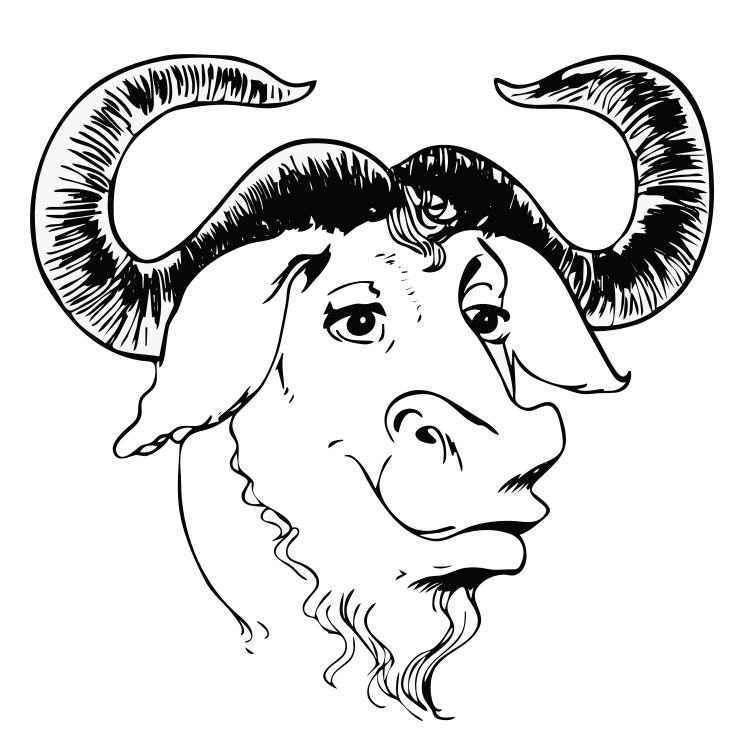
\includegraphics[height=40mm]{img/portada/gnu}
			
\includegraphics[height=40mm]{img/portada/bsd}
		\end{figure}
		% autor
		\vspace{20mm}
		Esteban De La Fuente Rubio \\
		\textit{esteban[at]delaf.cl} \\
		% fecha de cuando fue compilado
		\vspace{10mm}
		\today
	\end{center}
\end{titlepage}

% PÁGINA EN BLANCO
\newpage
\mbox{}
\thispagestyle{empty}


% páginas que no son parte del contenido del libro en números romanos
\frontmatter

% LICENCIA
%
% Apunte de Sistemas Operativos
% Copyright (C) 2014 Esteban De La Fuente Rubio (esteban[at]delaf.cl)
%
% Permission is granted to copy, distribute and/or modify this document
% under the terms of the GNU Free Documentation License, Version 1.3
% or any later version published by the Free Software Foundation;
% with no Invariant Sections, no Front-Cover Texts, and no Back-Cover Texts.
% A copy of the license is included in the section entitled "GNU
% Free Documentation License".
%
% Link: http://www.gnu.org/copyleft/fdl.html
%  

% LICENCIA
\chapter*{Licencia de uso}
\pagenumbering{roman}

Este documento se encuentra bajo la licencia de documentación libre GNU o GFDL.
A continuación se indican las condiciones generales respecto al uso de este
documento, una versión oficial (en inglés) y una traducción no oficial.

\begin{verbatim}
Copyright (c) 2014 Esteban De La Fuente Rubio
Permission is granted to copy, distribute and/or modify this document
under the terms of the GNU Free Documentation License, Version 1.3
or any later version published by the Free Software Foundation;
with no Invariant Sections, no Front-Cover Texts, and no Back-Cover Texts.
\end{verbatim}

\begin{verbatim}
Copyright (C) 2014 Esteban De la Fuente Rubio
Se autoriza la copia, distribución y/o modificación de este documento
bajo los términos de la Licencia de documentación libre de GNU, Versión 1.3
o cualquiera posterior publicada por la Fundación para el Software Libre;
sin secciones invariantes, ni textos de portada, ni textos de contraportada.
\end{verbatim}

Una copia de esta licencia puede ser encontrada (en inglés) en la siguiente
dirección: \url{http://www.gnu.org/licenses/fdl-1.3.txt}.

% PÁGINA EN BLANCO
\newpage
\mbox{}
\thispagestyle{empty}

% AGRADECIMIENTOS
%
% Apunte de Sistemas Operativos
% Copyright (C) 2014 Esteban De La Fuente Rubio (esteban[at]delaf.cl)
%
% Permission is granted to copy, distribute and/or modify this document
% under the terms of the GNU Free Documentation License, Version 1.3
% or any later version published by the Free Software Foundation;
% with no Invariant Sections, no Front-Cover Texts, and no Back-Cover Texts.
% A copy of the license is included in the section entitled "GNU
% Free Documentation License".
%
% Link: http://www.gnu.org/copyleft/fdl.html
% 

% AGRADECIMIENTOS
\chapter*{Agradecimientos}
Son varias las personas que me han ayudado y apoyado durante los años, varios
durante el tiempo que llevo escribiendo este apunte, y justamente gracias a
algunos de ellos es que decidí escribirlo en ``formato libro''. Algunos son:

Al profesor Gabriel Astudillo, ya que con su apoyo y motivación fomentó en mi la
parte práctica en sistemas operativos \textit{like Unix}.

Al profesor Carlos Abarzúa, quién fue la persona que me introdujo en el área de
teoría de los sistemas operativos.

Al profesor Guillermo Badillo, quién confió en mi por primera vez para dictar el
curso de Sistemas Operativos en la Universidad Andrés Bello.

Al profesor Luis Mateu, quién me aceptó como oyente\footnote{Fui oyente en otoño
2012, su alumno en otoño 2013 y su auxiliar en primavera 2013.} en sus clases de
Sistemas Operativos en la Universidad de Chile y en cuyas clases se basó gran
parte de este documento.

Además quisiera agradecer a todos aquellos que han permitido que este proyecto
salga adelante, ya sea con sus aportes, su ánimo o su paciencia (sobre todo
alumnos).

Adicionalmente agradeceré a cualquier lector que me indique sugerencias sobre el
contenido, reportes de errores o solicitud de algún tema que haya sido omitido o
no cubierto en la profundidad esperada. La idea es evaluar estos comentarios y
hacer los respectivos cambios en futuras versiones del documento.

% PÁGINA EN BLANCO
\newpage
\mbox{}
\thispagestyle{empty}

% RESUMEN
%
% Apunte de Sistemas Operativos
% Copyright (C) 2014 Esteban De La Fuente Rubio (esteban[at]delaf.cl)
%
% Permission is granted to copy, distribute and/or modify this document
% under the terms of the GNU Free Documentation License, Version 1.3
% or any later version published by the Free Software Foundation;
% with no Invariant Sections, no Front-Cover Texts, and no Back-Cover Texts.
% A copy of the license is included in the section entitled "GNU
% Free Documentation License".
%
% Link: http://www.gnu.org/copyleft/fdl.html
% 

% RESUMEN
\chapter*{Resumen}
Este documento tiene por objetivo presentar de manera sencilla los principales
conceptos relacionados con los Sistemas Operativos. Para lograr esto se
introducirá al lector en distintos temas, cubriendo tópicos desde los inicios de
los sistemas operativos hasta sistemas operativos modernos.

Es importante destacar que la motivación al escribir este documento es que pueda
servir como guía para quién se está introduciendo en conceptos relacionados al
área de Sistemas Operativos o bien esté tomando un curso de introducción a los
sistemas operativos donde la mayor parte de los temas mencionados en este
documento son utilizados.

Al ir avanzando en el documento el lector se irá adentrando, básicamente, en las
áreas de gestión de procesos, memoria principal y memoria secundaria. Para
lograr esto se cubren aspectos tanto teóricos como prácticos, esto último en
sistemas operativos \textit{like Unix}, como GNU/Linux.

El presente material está realizado en base a conocimientos adquiridos a lo
largo de los años, material de otros profesores que he tenido la suerte de
conocer y bibliografía de autores reconocidos en la materia. No se pretende que
este documento reemplace otras alternativas bibliográficas que el lector pueda
consultar, solo se presenta como un apunte para aquellos interesados en el
tema.

En \url{https://github.com/cursos/sistemas-operativos} el lector podrá encontrar
una copia digital, actualizada y gratuita de este documento.

% PÁGINA EN BLANCO
\newpage
\mbox{}
\thispagestyle{empty}


% ÍNDICE
\tableofcontents
\listoffigures
\addcontentsline{toc}{chapter}{Índice de figuras}
\listoftables
\addcontentsline{toc}{chapter}{Índice de cuadros}

% desde aquí parte la pagina número 1
\mainmatter
\pagenumbering{arabic}

% CAPÍTULO 1: INTRODUCCIÓN
%
% Apunte de Sistemas Operativos
% Copyright (C) 2014 Esteban De La Fuente Rubio (esteban[at]delaf.cl)
%
% Permission is granted to copy, distribute and/or modify this document
% under the terms of the GNU Free Documentation License, Version 1.3
% or any later version published by the Free Software Foundation;
% with no Invariant Sections, no Front-Cover Texts, and no Back-Cover Texts.
% A copy of the license is included in the section entitled "GNU
% Free Documentation License".
%
% Link: http://www.gnu.org/copyleft/fdl.html
%

% CAPÍTULO INTRODUCCIÓN
\chapter{Introducción}
El Sistema Operativo (\textit{Operating System, OS}) corresponde a un programa
en ejecución que se encarga de actuar como intermediario entre el usuario y la
máquina. Sus dos principales objetivos corresponden a la \textbf{administración
del hardware} y \textbf{ser una interfaz para el usuario}, de tal forma que este
pueda interactuar con la máquina.

El sistema operativo deberá proveer de un ambiente para ejecutar los programas
del usuario, siendo este \textbf{el único con privilegios de acceso directo al
hardware} y los procesos deberán mediante el sistema operativo acceder a los
recursos disponibles.

Los principales requisitos que se piden al sistema operativo corresponden a ser
\textbf{cómodo} en cuanto a su interfaz y \textbf{eficiente}, de tal forma que
no utilice todos los recursos de la máquina, dejándolos \textit{libres} para los
procesos de los usuarios.

Al estudiar la historia de los sistemas operativos se podrá apreciar como estos
han ido evolucionando en el tiempo. Se verá que inicialmente no existía un
sistema operativo como tal, sino que el hardware era programado directamente
recibiendo los trabajos (\textit{jobs}) que los usuarios deseaban ejecutar. Más
adelante, al aparecer el concepto de un monitor residente, se verá que este
corresponde a un programa que \textbf{siempre se encuentra cargado en memoria
principal}.

\section{Visión general}

En la figura \ref{fig:vision_global} se puede apreciar una visión global del
sistema operativo, en esta se muestran las principales partes que se verán en el
sistema. A continuación se describirá cada uno de estos componentes y como es la
interacción que estos tienen entre sí.

\begin{itemize}

	\item \textbf{Hardware}: recursos disponibles en la máquina, también
	podrán ser dispositivos virtuales, por estos los procesos competirán y
	desearán su uso.

	\item \textbf{Drivers}: código que permite el uso del hardware (o
	dispositivo virtual) al que están asociados.

	\item \textbf{Núcleo}: componente principal del sistema operativo, es el
	intermediario entre aplicaciones y el hardware, se encarga de las tareas
	de administración de la máquina.

	\item \textbf{Llamadas al sistema}: es la forma en que una aplicación
	hace alguna solicitud a un servicio del sistema operativo, generalmente
	con acceso privilegiado por lo cual son accedidas mediante una API.

	\item \textbf{API}: corresponde a una interfaz que pueden utilizar las
	aplicaciones para interactuar con el sistema operativo, las llamadas al
	sistema y eventualmente el hardware disponible, algunas ventajas de esto
	son la abstracción y el escribir menos código.

	\item \textbf{Utilitarios}: aquellas aplicaciones que vienen incluídas
	con el sistema operativo al momento de realizar la instalación, sin
	embargo esto dependerá mucho del sistema operativo propiamente tal y del
	contexto en que cada uno se instala.

	\item \textbf{Aplicaciones}: corresponden al software que se instala
	posteriormente a la instalación del sistema operativo. Generalmente
	serán las aplicaciones que principalmente le interesa ejecutar al
	usuario.

	\item \textbf{Usuario}: usuario del equipo que esta interesado en
	ejecutar sus aplicaciones.

\end{itemize}

\begin{figure}[htbp]
\centering
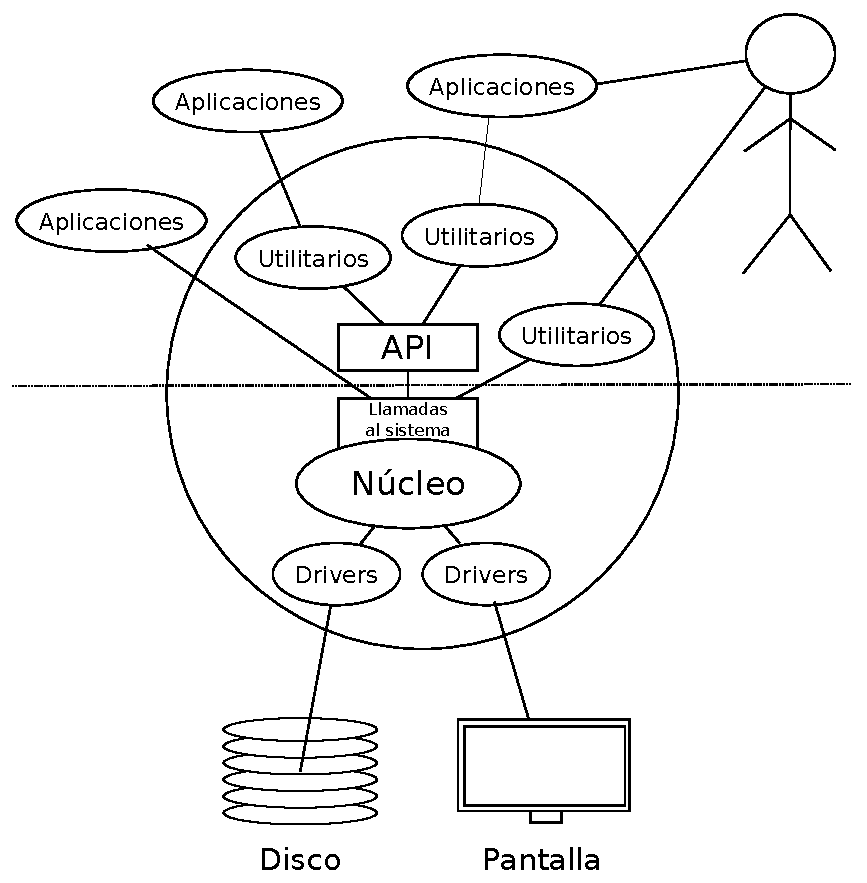
\includegraphics[scale=1.0]{img/C01_introduccion/vision_global.pdf}
\caption{Visión global del Sistema Operativo}
\label{fig:vision_global}
\end{figure}
\FloatBarrier

En la figura \ref{fig:vision_global} se observa una línea divisora entre los
componentes superiores (Aplicaciones, Utilitarios y API) y la parte inferior
(Llamadas al sistema, Núcleo, Drivers y Hardware). Esta división corresponde a
la separación de privilegios necesarios para ser utilizadas. Si bien una
aplicación podría acceder directamente a una llamada a sistema o al hardware
(\textbf{en Unix todo es un archivo}, incluso el hardware) deberá tener los
permisos adecuados para hacerlo. Se hablará más al respecto más adelante en el
capítulo \ref{estructura}.

Una característica importante del sistema operativo, como ya se mencionó antes,
es que es el único proceso que debe estar siempre cargado en memoria principal.
Lo anterior implicará que todo el código del sistema operativo, incluyendo sus
drivers deberán estar cargados siempre en RAM. Imagine que desea tener soporte
para todos los tipos de impresoras disponibles, esto implicaría tener cargado
todos los drivers en la memoria principal por si en algún momento usted la
conecta. Son parte de la estructura del sistema operativo y su diseño la
consideración de diferentes métodos de construcción del núcleo del sistema
operativo, lo que permita cargar por \textit{partes} el mismo, sin tener que
tener cargado todo el código que eventualmente se pueda requerir en la memoria.
Una de estas alternativas es lo que se utiliza en Linux, correspondiente al uso
de módulos donde el núcleo los levanta a medida que los requiere. De esto
también se hablará más en el capítulo \ref{linux_modulos}.

Si bien los recursos con los que se cuenta hoy en día son muy superiores a los
que se contaba cuando comenzaron los sistemas operativos, como se comentará en
el capítulo \ref{historia}, tenga en cuenta que la teoría de sistemas operativos
asociada a los conceptos que se verán en este apunte es muy similar. Existen
avances en tecnologías, pero lo que se abordará en este documento corresponde a
lo tradicional relacionado con sistemas operativos. Por lo cual si usted no
considera problema tener cargado 5, 15, 30 o 200 MB de núcleo RAM, recuerde que
hace unos años los equipos no tenían las mismas capacidades y hace décadas eran
impensables.

\section{Objetivos del sistema operativo}

El sistema operativo debe preocuparse de cumplir diferentes objetivos, estos se
pueden dividir, según el interesado, en \textbf{objetivos del usuario} y
\textbf{objetivos del sistema}.

\subsection{Objetivos del usuario}

Los usuarios finales en general no desean preocuparse por que tipo de hardware
están utilizando. Un usuario que quiere guardar una fotografía en su computador
no le interesa saber en que disco se esta guardando, de que tipo es el disco
(IDE o Sata) o que tipo de sistema de archivos contiene (ext3, reiserfs o xfs),
al usuario le interesa guardar la fotografía.

El objetivo de los desarrolladores estará asociado al fácil desarrollo de
aplicaciones sobre el sistema operativo. Sin tener que, el programador de la
aplicación, llegar a trabajar con lenguaje de bajo nivel o instrucciones
privilegiadas para acceder al hardware de la máquina.

Servicios que serán de interés para los usuarios:
\begin{itemize}

	\item \textbf{Creación de programas}: herramientas para realizar las
	tareas de desarrollo de aplicaciones para el sistema operativo.

	\item \textbf{Ejecución de programas}: administración de los procesos
	que se ejecutan en el sistema.

	\item \textbf{Acceso a los dispositivos de E/S}: simplificación de las
	tareas de uso del hardware, tales como escribir en una pantalla o leer
	datos desde el teclado.

	\item \textbf{Almacenamiento}: administración de los discos, la búsqueda
	de información en estos, su formato y gestión en general.

	\item \textbf{Memoria}: administración del uso de memoria principal
	disponible, así como la asignación de memoria virtual de ser necesario.

	\item \textbf{Detección y respuesta contra errores}: que sea capaz de
	detectar y proteger al sistema frente a eventuales anomalías.

	\item \textbf{Estadísticas}: llevar una recopilación con información
	sobre el uso de los recursos y parámetros generales sobre el sistema.

\end{itemize}

\subsection{Objetivos del sistema}

Desde el punto de vista del sistema la principal preocupación es realizar una
administración eficiente y justa de los recursos de la máquina. Esto significa
que todos sean atendidos en algún momento de tal forma que se les permita
realizar sus operaciones de forma satisfactoria.

El sistema operativo será el encargado de determinar cuando y quién utilizará
cierto recurso del sistema, tal como el procesador, la memoria principal, disco
duro, etc. Y será el encargado de interrumpir al proceso que haga uso del
recurso de tal manera de entregárselo a otro que también lo quiera utilizar.

\section{Servicios ofrecidos}
Históricamente se estudian principalmente tres áreas de la gestión realizada por
el sistema operativo, aquellas relacionadas con los procesos, memoria principal
y secundaria. Adicionalmente se verán en este documento otros aspectos como
protección y seguridad.

\subsection{Gestión de procesos}
Un \textbf{proceso corresponde a un programa en ejecución}, el cual posee
diferentes estados a lo largo de su vida como proceso. Principalmente interesan
los estados listos y ejecución, que corresponden a la espera antes de ser
planificado para entrar a la CPU y el de ejecución de código dentro de la CPU.
Existen otros estados que serán vistos en detalle en el capítulo
\ref{procesos}.

Todo proceso requerirá hacer uso de, al menos, memoria principal y CPU para su
ejecución, por lo cual el sistema operativo deberá ser capaz de asignar estos
recursos de una forma eficiente y justa, de tal forma que todos los procesos
sean servidos según los vayan requiriendo.

Se estudiarán problemas que ocurren por la ejecución de múltiples procesos al
mismo tiempo, concepto conocido como concurrencia, la forma de solucionarlo
mediante sincronización, y algoritmos de planificación que permitirán elegir que
proceso deberá entrar a al cpu.

\subsection{Gestión de memoria principal}
Todo proceso requerirá del uso de memoria principal para su ejecución, en este
espacio de memoria se encontrará no solo el código del programa, sino también
sus datos y su contexto. El sistema operativo deberá asignar, de algún modo,
espacios de memoria para que el proceso los utilice, y si eventualmente el
proceso requiere más espacio poder cumplir con su requerimiento.

¿Qué sucede si no disponemos de más memoria principal? La primera idea, sería
decir que no podemos iniciar más procesos, lo cual sería cierto, sin embargo se
discutirá el método de memoria virtual el cual permite utilizar un dispositivo
de memoria secundaria para ``obtener memoria'' para los procesos.

\subsection{Gestión de memoria secundaria}
El sistema operativo debe ser capaz de almacenar datos en medios de memoria
secundaria, la cual es permanente, a diferencia de la memoria principal que es
volátil. Se deberá preocupar de la mantención de una estructura de archivos y de
poder realizar operaciones sobre esta estructura de tal forma que las
aplicaciones no se preocupen de escribir \textit{físicamente} el archivo que
desean guardar en el disco.

\section{Ejercicios y preguntas}
\begin{enumerate}

	\item Explique los objetivos del sistema operativo.

	\item Explique los componentes de la visión general del sistema
	operativo y como se relacionan entre si. Realice diagrama.

	\item ¿Por qué los objetivos del usuario y del sistema operativo no
	siempre son compatibles?.

	\item ¿Cuáles son los servicios básicos que el sistema operativo debe
	proveer?.

	\item ¿Cuándo se encuentra cargado el sistema operativo en RAM?.

\end{enumerate}

\section{Referencias}
\begin{itemize}

	\item Sistemas Operativos, Segunda Edición, Andrew Tanenbaum, Capítulo 1.1.

\end{itemize}


% CAPÍTULO 2: HISTORIA
%
% Apunte de Sistemas Operativos
% Copyright (C) 2014 Esteban De La Fuente Rubio (esteban[at]delaf.cl)
%
% Permission is granted to copy, distribute and/or modify this document
% under the terms of the GNU Free Documentation License, Version 1.3
% or any later version published by the Free Software Foundation;
% with no Invariant Sections, no Front-Cover Texts, and no Back-Cover Texts.
% A copy of the license is included in the section entitled "GNU
% Free Documentation License".
%
% Link: http://www.gnu.org/copyleft/fdl.html
%

% CAPÍTULO HISTORIA
\chapter{Historia}
\label{historia}
Los sistemas operativos han evolucionado enormemente desde sus inicios, durante
este capítulo se mencionarán aspectos relacionados con los diferentes tipos de
sistemas operativos existentes o que han existido junto a lo que se ha logrado a
lo largo de los años.

\section{Tipos de sistemas}

\subsection{Érase una vez (50's)}
Cuando se comenzaron a utilizar grandes máquinas para realizar cómputos no
existía un sistema operativo propiamente tal, solo había hardware y las
aplicaciones (trabajos o \textit{jobs}) de los usuarios. Se leía el programa a
ejecutar y se ejecutaban sus instrucciones de manera secuencial.

Las aplicaciones en esta época debían incluir todo el código, incluyendo aquel
para manejar cada uno de los dispositivos de hardware que la máquina tenía
disponible. Se debe acceder directamente al espacio de direcciones, tanto de
memoria principal como memoria secundaria. No existe estructura de directorios
ni archivos en la memoria.

Si se desea ejecutar una nueva aplicación, se debe cargar el nuevo trabajo y la
máquina debe ser reiniciada. La depuración de la aplicación se realiza de forma
presencial, observando las salidas indicadas mediante las luces del computador.
El equipo es utilizado solo por un usuario al mismo tiempo y por un período
largo de tiempo para realizar todas las tareas involucradas.

El principal problema de esta etapa es el bajo uso del hardware disponible,
donde existe mucho tiempo que no es utilizado en cómputo. Siendo que el
componente caro es el hardware y no el programador, se debe buscar una solución
a este problema.

A pesar de lo anterior, y lo rudimentario que podría parecer frente a los
computadores que actualmente existen, estas máquinas eran capaces de procesar
cálculos mucho más rápido que un gran número de calculistas trabajando en
conjunto.

\subsection{Sistemas por lotes (fines 50's)}
En un sistema operativo por lotes se requiere que todos los componentes del
programa, ya sea el mismo código del programa, los datos y las llamadas al
sistema que permiten usar el hardware sean introducidos, comúnmente, mediante
tarjetas perforadas, ver figura \ref{fig:lotes}, de 80 caracteres cada una. Este
conjunto de instrucciones es conocido como un trabajo o un \textit{job}, el cual
poseía poca o ninguna interacción con el usuario.

\begin{figure}[htbp]
\centering
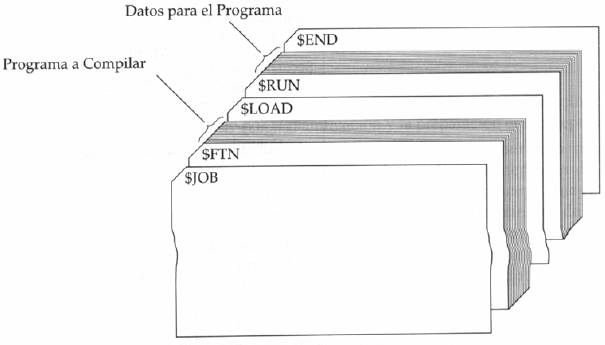
\includegraphics[scale=.7]{img/C02_historia/lotes.png}
\caption{Tarjetas de un sistema por lotes}
\label{fig:lotes}
\end{figure}

Este tipo de sistemas operativos era útil con programas que fuesen largos y sin
interacción con el usuario. Donde un operador recibía los trabajos de los
programadores y los introducía en la máquina, estos eran procesados en orden
FIFO (First In First Out), o sea el primer trabajo que llegaba era el primero
que se procesaba.

La planificación del procesador y administración de la memoria es simple, en el
primer caso bastaba pasar el control del mismo al \textit{job} y que este lo
devolviera al terminar su ejecución. En el caso de la memoria también la
administración era simple, ya que el espacio se dividía en dos partes, una para
el monitor residente (el sistema operativo) y otra para el trabajo en
ejecución.

Al aparecer el monitor residente, también aparece el concepto de API, donde el
programador ya no debía escribir todas las instrucciones para acceder al
hardware, sino que se le entregaba ya una herramienta para facilitar su
trabajo.

Si ocurría algún error durante la ejecución del trabajo se entregaba al
programador un \textit{dump} de la memoria, de tal forma que este pudiera
corregir el error en el programa y volver a entregar un conjunto de tarjetas
corregidas para su ejecución. Esto evitaba que el programador tuviese que estar
frente al computador para depurar su código.

A pesar de que el computador se encontraba más tiempo ocupado, porque siempre
que hubiesen tarjetas se estarían procesando, su componente más costosa, la CPU,
que es más rápida comparada con los dispositivos de entrada o salida de datos,
no se encontraba necesariamente ocupada todo el tiempo. Las tareas de lectura y
escritura son bloqueantes y mantienen a la CPU en un ciclo de
\textit{busy-waiting}. Lo anterior significa que mientras se está leyendo o
escribiendo, la CPU no puede realizar otras tareas (ya que espera que la lectura
o escritura termine).

\subsection{Sistemas de operación \textit{offline} (60's)}
La idea principal tras las operaciones fuera de línea, o \textit{offline},
corresponde a la lectura y escritura de los elementos utilizados en los sistemas
operativos por lotes, o sea las tarjetas, de forma externa al computador
principal. Lo anterior buscaba no utilizar el procesador más caro disponible en
tareas lentas (como leer tarjetas), sino utilizar otras unidades que traspasaban
las tarjetas perforadas a cintas y luego estas cintas eran cargadas en la
máquina principal.

Análogamente a lo explicado, la salida del computador principal era generada en
cintas magnéticas, las cuales en una etapa posterior a la ejecución del programa
eran llevadas a un equipo de impresión donde se obtenía una salida que se
entregaba al programador.

Con este sistema fuera de línea, se lograba un mejor rendimiento del procesador
principal, utilizándolo para tareas de cómputo y dejando las tareas de lectura y
escritura a otros equipos más económicos.

La cantidad de máquinas periféricas utilizadas dependerá de la capacidad del
procesador, o sea, mientras existiera tiempo de CPU sin uso, se podían seguir
agregando cintas al computador principal. Una vez el tiempo de CPU ya había
alcanzado su uso constante, no tenía sentido agregar más impresoras (o lectoras)
ya que no se generarían más cintas para imprimir por unidad de tiempo.

El trabajo solo entrega el control del sistema al monitor residente en caso de
término, que se requiera algún servicio de entrada o salida o en caso de error.

A pesar de esta mejora en la velocidad de lectura y escritura, el procesador,
mientras se realizan dichas operaciones, continúa estando ocioso, sigue
existiendo problema de \textit{busy-waiting} en cintas. Consideremos que para
leer una línea de la cinta se tomaban 80 caracteres (misma cantidad que una
tarjeta perforada) y se escribían de a 80 caracteres (en caso de cintas) y de a
132 caracteres en impresoras. El leer una línea implicaba hacer girar la cinta,
lo cual generaba inercia en la cinta y hacía que hubiese que ajustarla
(retrocediendo) para leer la próxima línea en el futuro.

Adicionalmente existía un mayor tiempo para los programadores, que debían
esperar que sus programas fueran traspasados a cinta, ejecutados, luego los
resultados traspasados a cinta e impresos.

\subsection{Sistemas con \textit{buffering} (60's)}
Para ayudar a solucionar el problema de leer línea a línea las instrucciones de
una cinta se empezaron a leer de a 10 líneas, o sea de a 800 caracteres, lo cual
permitía disminuir los tiempos de lectura. En vez de leer de a una línea, se
leían 10 considerando que en algún momento futuro esas líneas podrían ser
utilizadas, las líneas leídas eran guardadas en un \textit{buffer} a la espera
de ser solicitadas. Por lo tanto cuando eventualmente el trabajo requería una
línea, esta era leída desde el \textit{buffer} y no desde la cinta, reduciendo
los tiempos.

De la misma forma para escribir en la cinta, se guardaba en un \textit{buffer}
lo que se quisiera escribir, una vez lleno este \textit{buffer} se escribía todo
en la cinta de una vez.

Mediante el uso de canales, uno para la lectura y otro para la escritura, se
podían conseguir mejoras en los tiempos y rendimiento de la CPU. Ya que la tarea
de leer y llevar al \textit{buffer} o sacar del \textit{buffer} y escribir la
realizaban los canales propiamente tal, y la CPU no era necesaria durante toda
la operación de E/S, con lo que la misma podía ser utilizada para tareas de
cómputo.

El rendimiento de esta técnica dependerá básicamente de si el proceso es
intensivo en CPU, en E/S o es igual en ambos casos. A pesar de lo anterior el
porcentaje de utilización de CPU, gracias al \textit{buffering} y uso de canales
aumentará.

El principal problema de esta técnica sigue siendo el tiempo de espera extra
agregado al tener que leer las tarjetas y cargarlas en cintas y luego las cintas
imprimirlas, esto básicamente por el transporte de un sistema periférico al
computador principal.

\subsection{Sistemas de operación \textit{online} (60's)}
En este tipo de sistemas la lectura de tarjetas e impresión de resultados ya no
es realizada en equipos periféricos. Las lectoras e impresoras se conectan
directamente al computador central y hacen uso de los canales de E/S que se
agregaron en el sistema con \textit{buffering}. Esto fue posible gracias a la
aparición de discos duros los cuales contenían la entrada de los trabajos y
almacenaban las salidas de los mismos.

En este tipo de sistemas el monitor residente es quien se encarga de leer
tarjetas y dejarlas en el disco y de imprimir los resultados. Para ejecutar un
trabajo debe haber sido leído completamente al disco, así mismo para imprimir
los resultados de un trabajo este debe haber terminado su ejecución habiendo
dejado la salida en el disco.

Esto mejora el tiempo de proceso de un trabajo, ya que no se deben utilizar
lectores o impresoras externas al computador principal, ahorrando tiempo en el
traspaso físico de las mismas de un equipo a otro.

El problema sigue siendo la ociosidad del procesador cuando se deben realizar
operaciones de entrada o salida.

\subsection{Sistemas multiprogramados (fines 60's)}
El principal problema con un sistema de operación \textit{online} es que la CPU
no está siendo utilizada todo el tiempo, esto a pesar que pueden existir
trabajos que pudiesen ser atendidos. Esto es básicamente porque no se permite la
ejecución de más de un trabajo en ``paralelo'' y se debe esperar a que uno
termine para iniciar otro.

En este tipo de sistemas se aprovecha el tiempo de E/S para ejecutar otros
trabajos. Durante esta época aparece el concepto de planificación de
procesos/trabajos (o \textit{scheduling}) y con esto el concepto de Sistema
Operativo. Ya que varios procesos deben ejecutarse, todos ellos deben estar
residentes en memoria principal. La multiprogramación implica multiprocesos, o
sea programas se ejecutan de forma ``paralela'', ver figura
\ref{fig:multiprogramado}.

\begin{figure}[htbp]
\centering
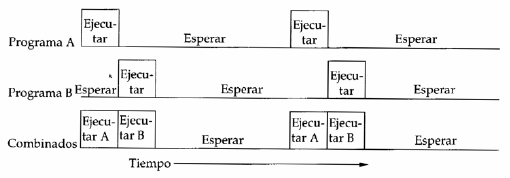
\includegraphics[scale=1.]{img/C02_historia/multiprogramacion.png}
\caption{Sistemas por lotes vs sistema multiprogramado}
\label{fig:multiprogramado}
\end{figure}

El principal problema es la no existencia de un entorno protegido para la
ejecución de los procesos, si un proceso cometía algún error podía hacer que
todo el sistema fallase.

\subsection{Máquinas o procesadores virtuales}
En este tipo de máquinas, se da soporte para la emulación de varias máquinas o
procesadores a partir de un solo procesador real. Cada máquina virtual entrega
al proceso un entorno protegido, frente a otras máquinas virtuales, de tal forma
que lo ejecutado en dicho entorno solo afecta a esa máquina virtual.

El tiempo de CPU utilizado por cada máquina es una tajada de tiempo del
procesador real. Con esto se logra el mayor rendimiento del computador,
utilizando multiprogramación, ya que la CPU siempre estará atendiendo a alguien
que lo requiera.

El problema aquí comienza a ser la baja productividad de los programadores. Lo
tiempos de ejecución total de un proceso sigue siendo alto, y la depuración de
los trabajos comienza a tomar importancia como problema.

\subsection{Sistemas de tiempo compartido (70's)}
Los sistemas de tiempo compartido corresponden a entornos multiprogramados y
multiusuario, los cuales entregaban un mejor tiempo de respuesta. Los usuarios
(programadores) pueden trabajar de forma interactiva con los computadores
mediante terminales conectadas a ellos. O sea, vuelven a trabajar directamente
con el computador, como lo hacían en los inicios, el operador ya no existe.

Cada programador dispone de una terminal con una consola, donde puede realizar
una depuración de forma más rápida, no debiendo esperar la entrega de los
resultados de la ejecución de su programa impresos.

En un sistema de tiempo compartido los usuarios comparten recursos, por lo cual
se debe hacer un reparto equitativo de los mismos y además contar con sistemas
de protección para ellos. Ahora se habla de sesiones de usuarios y no de
trabajos.

El problema aquí surge con la cantidad de usuarios y procesos que estos
ejecutan, donde el procesador no es capaz de atender a infinitos usuarios y el
sistema puede ir degradándose con cada nuevo que entra. Esto ya que el recurso
CPU que realiza los cómputos y el recurso memoria que se requiere para mantener
los procesos en ejecución son limitados.

\subsection{Computadores personales}
Gracias al uso de componentes cada vez más pequeños se logró empezar a
comercializar microprocesadores, los cuales permitían, por su bajo costo, que
fuesen adquiridos por usuarios personales. De esta forma ya no se requería
compartir el recurso CPU o memoria con múltiples usuarios, sino que cada usuario
(o programador) disponía de un equipo dedicado a sus labores.

Originalmente los computadores personales, destinados al uso por parte de un
único usuario, no requerían características de sistemas de tiempo compartido.
Con esto su diseño era más simple y requerían menos soporte del hardware para su
funcionamiento. Un ejemplo de este tipo de sistema operativo es MS-DOS.

Cada usuario posee su propia máquina, sin embargo el compartir datos entre
máquinas resultaba un proceso complicado. Cada máquina debía tener su propia
impresora y/o lectora de discos.

\subsection{Redes de computadores personales (80's)}
A mediados de los 80's surgen las redes de computadores personales, bajo esta
modalidad los usuarios podían compartir discos e impresoras con otros equipos y
de esta forma economizar en la compra de recursos.

Este esquema utiliza uno de los equipos como servidor de disco y/o impresora, y
los demás computadores se conectan vía red a este. Los usuarios conectados a
estas terminales, veían el disco o la impresora como si estuviese conectada en
su equipo.

Ya que el sistema operativo utilizado, en realidad un monitor residente, no
poseía características de protección es que era poco recomendable ejecutar
aplicaciones de usuario en el servidor, ya que la caída de la aplicación podría
hacer que todo el sistema fallase.

Las primeras redes solo permitían compartir directorios en modo solo lectura.

\subsection{Sistemas en tiempo real}
Este tipo de sistemas corresponde a los utilizados en aplicaciones de tiempo
real, donde los tiempos de respuesta a eventos del mundo físico son críticos.
Por ejemplo el uso en control de tráfico o procesos industriales.

Deben poseer tiempo de respuestas muy rápidos, para esto es requisito que los
procesos residan permanentemente en memoria principal. Adicionalmente cualquier
interrupción debe ser atendida inmediatamente. No se garantiza que se reciba de
forma inmediata, pero si en un tiempo muy acotado.

Existen variantes de GNU/Linux que están orientadas a sistemas operativos en
tiempo real.

\subsection{Sistemas distribuídos}
Corresponden a un conjunto de estaciones de trabajo o \textit{terminales
inteligentes} conectadas entre sí para trabajar de manera conjunta y como una
sola. Este modo de operación ha sido influenciado por el decaimiento del costo
de los procesadores, donde es más barato tener dos CPU funcionando conjuntamente
que una sola CPU del doble de velocidad.

Se hace uso de las redes de computadores, donde cada nodo de la red es una pieza
del computador conformado. Con esto se consigue una serie de ventajas tales como
alto rendimiento, alta disponibilidad, balanceo de carga y escalabilidad.

\subsection{Sistemas multiprocesadores}
Un sistema con múltiples procesadores permite la ejecución real en paralelo de
al menos dos procesos, considerando que como mínimo existirán dos procesadores.
En estricto rigor, y por definición de Intel, son \textit{cores} o (núcleos),
donde un procesador puede tener uno o más \textit{cores}. Quedando el concepto
de procesador o CPU como el chip y \textit{core} como el componente de la CPU
que ejecuta los procesos.

Cuando el número de procesos en ejecución supera el número de \textit{cores} se
debe recurrir al uso de algún mecanismo de planificación de procesos, donde se
deberá, al igual que en sistema monoprocesador, compartir el tiempo de CPU entre
los interesados.

Se hablará de tiempo de CPU durante el texto, pero recordar que nos estaremos
refiriendo a los \textit{cores} que están en la CPU.

\section{Tendencias últimas dos décadas}

Durante las últimas dos décadas, o sea desde los 90's, han existido diversas
tendencias en lo referente al desarrollo de sistemas operativos.

El gran crecimiento que han experimentado las redes computacionales junto a las
velocidades de acceso a Internet han permitido un mayor uso de computación
distribuida, mediante el uso de plataformas multiprocesadoras y procesadores
conectados en red.

El área de sistemas multimedia, datos más sonido más imágenes ha experimentado
un alto desarrollo. Se están desarrollando cada vez dispositivos de entrada más
rápidos y eficientes como los sistemas de reconocimiento automático de voz o
imágenes. Dichos sistemas tienen directa relación con los mencionados como
sistemas de tiempo real.

Adicionalmente la tendencia va hacia el diseño e implementación de sistemas
abiertos, tales como:

\begin{itemize}

	\item Normas de comunicación abiertas, como el modelo de referencia OSI.

	\item Normas de Sistemas Operativos abiertos como GNU/Linux.

	\item Normas de interfaces de usuario abiertas, como el sistema de
	ventanas X desarrollado por MIT.

	\item Normas de aplicaciones de usuario abiertas, como las entregadas
	por la FSF\footnote{Free Software Foundation /
	\url{http://www.gnu.org/licenses/gpl.html}}.

\end{itemize}

\section{Logros}
Durante los años de desarrollo se han obtenido diferentes logros, que perduran
en los sistemas hasta hoy en día. A continuación se mencionan brevemente estos,
en capítulos posteriores se discutirá en detalle cada uno de ellos.

\subsection{Procesos y memoria}
Un proceso corresponde, en principio, a cualquier programa en ejecución. Este
posee diversos estados, donde lo más común es encontrar: ejecución (proceso en
cpu), bloqueado (en espera de un recurso) y listo (esperando entrar a cpu).

Cualquier proceso requerirá si o si al menos el uso de memoria principal y CPU,
adicionalmente puede requerir utilizar otros dispositivos, en general cualquiera
destinado a operaciones de entrada y salida. Esto implicará que diversos
procesos podrán tratar de acceder a un mismo recurso al mismo tiempo, por lo
cual existirá competencia por dicho recurso. Para esto, a lo largo de los años,
se han diseñado diversos algoritmos que permiten al sistema operativo decidir
que proceso utilizará que recurso.

Además un proceso para funcionar requerirá algo más que su código, un proceso
estará formado por el programa o código, sus datos y un contexto (o descriptor
del proceso).

Finalmente el sistema operativo debe ser capaz de prevenir o mitigar los
problemas más comunes correspondientes a \textit{data races}, \textit{deadlock}
y \textit{starvation}. Para esto, existen mecanismos de sincronización que se
pueden utilizar.

\subsection{Seguridad y protección}
Se debe garantizar la protección de los procesos en ejecución, se mencionó ya
que sistemas operativos de tiempo compartido debían proteger a los procesos
corriendo, ya que múltiples usuarios podrían estar trabajando en la máquina.
Específicamente se deben implementar políticas que permitan controlar el acceso
a un recurso solicitado por más de un proceso, a este recurso se le conocerá
como \textbf{sección crítica} y algunas medidas que se pueden tomar son:

\begin{itemize}

	\item No compartición: procesos se encuentran aislados.

	\item Compartición solo como lectura, para escribir un recurso se
	requieren mecanismos (o condiciones) especiales.

	\item Subsistemas confinados: similar a una protección por ocultación
	donde un proceso evita que otros sepan como opera.

	\item Diseminación controlada: en este caso existen credenciales de
	seguridad para acceder a los recursos, por lo cual se especifica quien
	podrá y quien no podrá acceder al recurso.

\end{itemize}

\subsection{Gestión de recursos}
La gestión de recursos corresponde a como se deberán asignar los recursos a un
proceso que los solicite, considerando para esto que deberá existir algún tipo
de planificación que determine el orden en que serán atendidas las solicitudes.
Se deben considerar los factores:

\begin{itemize}

	\item Equidad: igualdad de preferencias frente a una solicitud.

	\item Sensibilidad: poder priorizar ciertos procesos.

	\item Eficiencia: maximizar la productividad y minimizar los tiempos de
	respuestas.

\end{itemize}

Más adelante se hablará de la planificación de CPU y como el sistema operativo
asigna este recurso a un proceso, se deberá considerar que conceptos mencionados
para la CPU son análogos a los utilizados en la planificación de otro tipo de
recursos.

\subsection{Estructura del sistema}
La estructura o arquitectura del sistema, determinará como se comportará y que
capacidades podrá el sistema operativo entregar a los procesos y usuarios que
están ejecutándose sobre el.

Es importante mencionar que la estructura del software utilizada dentro del
sistema operativo puede afectar considerablemente el funcionamiento de este. No
será lo mismo una rutina programada de cierta forma que de otra, una puede ser
más o menos eficiente dependiendo de la implementación realizada. Así mismo un
sistema con más o menos instrucciones no significa que sea un sistema más o
menos eficiente, ni mucho menos más o menos simple. Ya se habrá visto en
lenguajes de programación que existen instrucciones que utilizan muy pocas
líneas, sin embargo son difícilmente entendibles.

Se deberá dividir el sistema operativo, de tal forma que cada una de las partes
de este cumpla una función específica. Si bien se puede tener un único sistema
que implemente todas las funcionalidades (este es el caso de un sistema
operativo monolítico), aun así internamente deberá estar organizado de tal forma
que sea sencillo de mantener y programar. De no realizarse lo anterior de forma
correcta podrían existir problemas con los tiempos de entrega del software,
fallos y rendimiento en el momento de poner en funcionamiento un nuevo sistema.

El capítulo \ref{estructura} discute los conceptos de la estructura del sistema
operativo en un nivel más profundo.

\section{Ejercicios y preguntas}
\begin{enumerate}

	\item ¿Cuándo es recomendable el sistema operativo por lotes?.

	\item Describa las ventajas de un sistema de operación \textit{offline}
	versus un sistema operativo por lotes.

	\item ¿Cuál es el problema de los sistemas de operación \textit{offline}
	que se soluciona en uno con \textit{buffering}?

	\item Indique la característica que hace a un sistema multiprogramado
	ser más eficiente que sus predecesores.

	\item En un sistema de tiempo compartido ¿cuántos usuarios pueden correr
	sus programas al mismo tiempo?.

	\item ¿Cuál es la principal característica de un sistema operativo en
	tiempo real?.

	\item ¿Quién inicio el proyecto GNU?.

	\item ¿Quién inicio el proyecto Linux?.

	\item ¿Cuáles son las 4 libertades que entrega el software libre?.

	\item ¿Qué es un proceso?.

	\item Un proceso ¿es solo código?.

	\item ¿Qué se conoce como sección crítica?.

	\item Explique los conceptos de equidad, sensibilidad y eficiencia.

\end{enumerate}

\section{Referencias}
\begin{itemize}

	\item Sistemas Operativos, Segunda Edición, Andrew Tanenbaum, Capítulo
	1.2.

	\item Sistemas Operativos, Quinta Edición, Abraham Silberschatz y Peter
	Baer Galvin, Capítulo 1.

	\item Sistemas Operativos, Segunda Edición, William Stallings, Capítulo
	2.

\end{itemize}


% CAPÍTULO 3: ESTRUCTURA Y DISEÑO
%
% Apunte de Sistemas Operativos
% Copyright (C) 2014 Esteban De La Fuente Rubio (esteban[at]delaf.cl)
%
% Permission is granted to copy, distribute and/or modify this document
% under the terms of the GNU Free Documentation License, Version 1.3
% or any later version published by the Free Software Foundation;
% with no Invariant Sections, no Front-Cover Texts, and no Back-Cover Texts.
% A copy of the license is included in the section entitled "GNU
% Free Documentation License".
%
% Link: http://www.gnu.org/copyleft/fdl.html
%

% CAPÍTULO ESTRUCTURA Y DISEÑO
\chapter{Estructura y diseño}
\label{estructura}
El sistema operativo es el encargado de ofrecer diferentes servicios, tanto al
usuario como a otros procesos. Es importante mencionar que aquí se contrapondrán
los objetivos que tiene el sistema con los requerimientos de los usuarios.

A continuación se listan una serie de servicios que deben ser considerados al
momento de diseñar un sistema operativo, algunos de los cuales se discutirán en
mayor detalle más adelante.

\begin{enumerate}[a.]

	\item \textbf{Interfaz de usuario}: servicio que entrega un método para
	que el usuario pueda interactuar con el sistema operativo, ya sea una
	CLI o una GUI.

	\item \textbf{Ejecución de programas}: el sistema operativo se debe
	encargar de mantener a los procesos en ejecución durante todo su ciclo
	de vida, esto implica la administración de los mismos durante sus
	posibles estados de ejecución.

	\item \textbf{Operaciones de entrada/salida (E/S)}: un proceso no podrá
	acceder directamente a los recursos disponibles en la máquina, debe ser
	el sistema operativo quien, mediante una interfaz de acceso, permita a
	los diferentes procesos acceder a los dispositivos de entrada y salida
	de forma concurrente y controlada.

	\item \textbf{Sistema de archivos}: se debe proveer de una forma de
	acceder al disco con alguna estructura, donde no se deban escribir
	directamente posiciones de memoria, sino que los procesos puedan
	escribir y leer archivos dentro de los dispositivos.

	\item \textbf{Comunicación entre procesos (IPC o \textit{Inter Process
	Communication})}: corresponde al mecanismo que permite que diferentes
	procesos se comuniquen entre sí, por ejemplo mediante el uso de memoria
	compartida, \textit{sockets} o tuberías.

	\item \textbf{Detección de errores}: sistema deberá capturar los
	errores, tanto físicos como lógicos que un proceso pueda generar y
	evitar que dicho error afecte a otros procesos en ejecución.

	\item \textbf{Asignación de recursos}: los diferentes dispositivos en la
	máquina podrán ser utilizados concurrentemente por muchos procesos, por
	lo que deberá existir algún algoritmo que permita planificar quien
	utilizará un recurso en un momento dado.

	\item \textbf{Estadísticas}: estas son llevadas con propósitos
	contables, para detectar errores o para, por ejemplo, predecir el
	comportamiento futuro de un proceso y poder tomar decisiones de
	planificación al respecto.

	\item \textbf{Protección y seguridad}: el acceso a los recursos
	disponibles debe ser controlado, se debe evitar que cualquier proceso
	pueda utilizar cualquier dispositivo, en cualquier momento.

\end{enumerate}

\section{Interfaz de usuario}
Las \textbf{interfaces de usuario} permiten al usuario realizar una interacción
con el sistema operativo, se dividen básicamente en dos tipos
\textbf{\textit{Command Line Interface}} (CLI) y \textbf{\textit{Graphical User
Interface}} (GUI).

\subsection{CLI}
La interfaz de línea de comando, o simplemente la \textit{shell}, corresponde a
un intérprete en modo texto que permite introducir órdenes para que sean
ejecutadas por el sistema operativo. Su tarea principal es recibir las
solicitudes del usuarios, y en la mamyoría de los casos ejecutar un programa
asociado a dicha solicitud.

Algunos ejemplos de \textit{shells} conocidas en diferentes sistemas operativos
\textit{like Unix} son:

\begin{itemize}

	\item sh: Steve Bourne, Unix v7, 1978.

	\item ash: usada como base para las shell de BSD.

	\item bash: parte del proyecto GNU.

	\item dash: ash mejorada para Debian GNU/Linux.

\end{itemize}

La \textit{shell} ejecutará los comandos que el usuario introduzca, algunos de
ellos serán comándos básicos (como listar directorios, crear una carpeta, ver la
fecha) o podrían ser programas más complejos (como un editor de texto o una
aplicación en modo texto). Adicionalmente se puede utilizar un lenguaje de
programación para realizar \textit{scripts}, donde existe un estándar denominado
\textit{shell scripting}, sin embargo cada intérprete puede implementar
extensiones para el mismo.

Un comando al ser ejecutado deberá ser buscado dentro del PATH del sistema, el
cual corresponde a la ruta de directorios donde posiblemente se podría encontrar
dicho comando, si luego de revisar todos los directorios del PATH el comando no
es encontrado se informa al usuario. En caso de ser encontrado el comando puede
estar implementado como un programa externo de la \textit{shell} o como un
programa dentro de la \textit{shell}, como el caso de algunas extensiones. La
ventaja de utilizar el primer método, fuera del intérprete, es que no se debe
modificar este para agregar nuevos comandos, bastará agregarlos a alguna de las
rutas en el PATH.

En general la shell de un usuario no privilegiado (usuario normal) tendrá el
signo \$ y un usuario privilegiado (o sea, el usuario root) tendrá el signo \#
para indicar que está en espera del ingreso de comandos. De esta forma si vemos
un comando precedido por un signo \$, dicho comando se ejecuta como usuario sin
privilegios, en cambio si vemos un comando precedido por un signo \#
necesariamente dicho comando se debe ejecutar con el usuario root.

\subsection{GUI}
La interfaz de usuario gráfica corresponde al entorno de ventanas, el cual
permite tener diversas aplicaciones encapsuladas dentro de un cuadro (ventana) y
de esta forma compartir de manera fácil un único recurso, la pantalla, con
múltiples procesos que quieren dibujar en ella. En sistemas \textit{like Unix}
es conocido como X en honor a Xerox que lo ideo en los años 70s\footnote{¡Si!
mucho antes que Microsoft Windows empezara a usarlas}.

Algunos entornos de escritorio y gestores de ventanas son KDE, Gnome, XFCE,
Lxde, Fluxbox y OpenBox. Algunos de estos pueden apreciarse en la figura
\ref{gui}.

El entorno gráfico no es propiamente una función del sistema operativo, de hecho
es una aplicación más que funciona sobre este, la cual entrega una forma ``más
amigable'' de interactuar con el sistema.

\begin{figure}[htbp]
\begin{center}
	\subfigure[KDE 3.5]{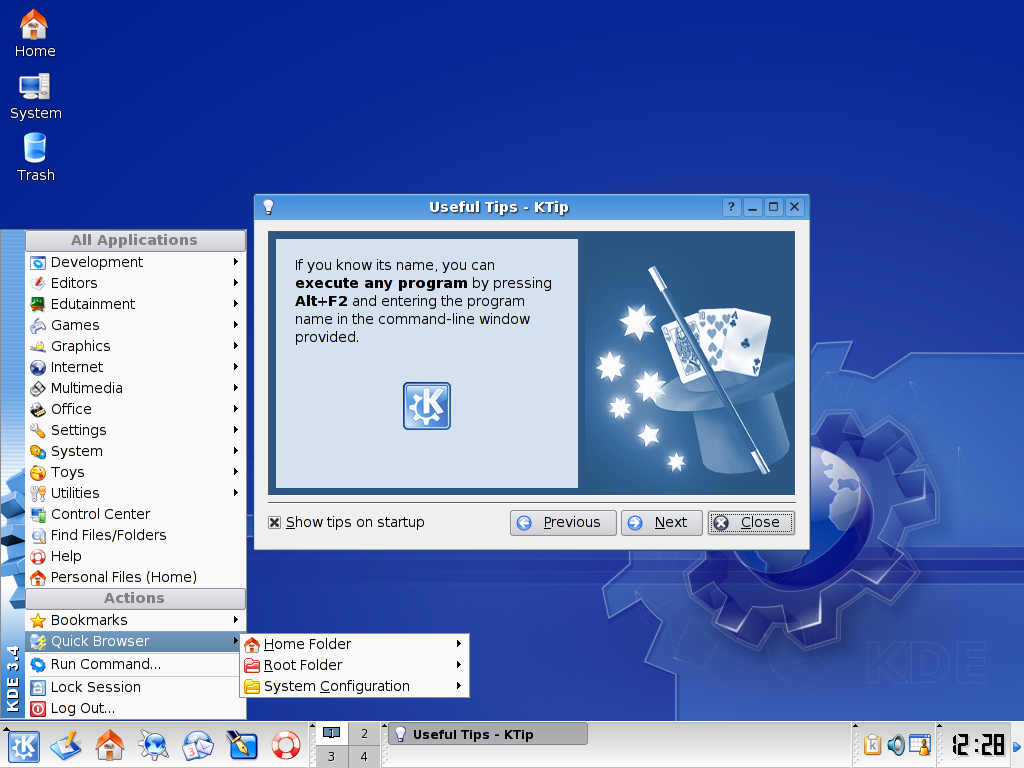
\includegraphics[height=3.5cm]{img/C03_estructura/gui_kde35}}
	\subfigure[KDE 4]{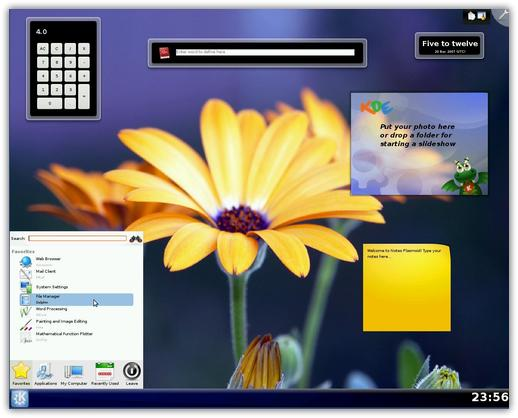
\includegraphics[height=3.5cm]{img/C03_estructura/gui_kde4}}
	\subfigure[Gnome]{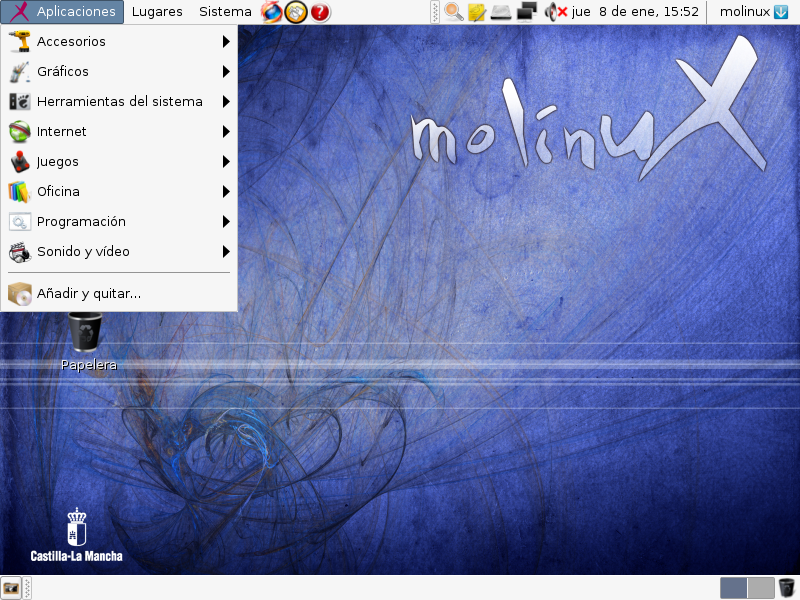
\includegraphics[height=3.5cm]{img/C03_estructura/gui_gnome}}
	\subfigure[XFCE]{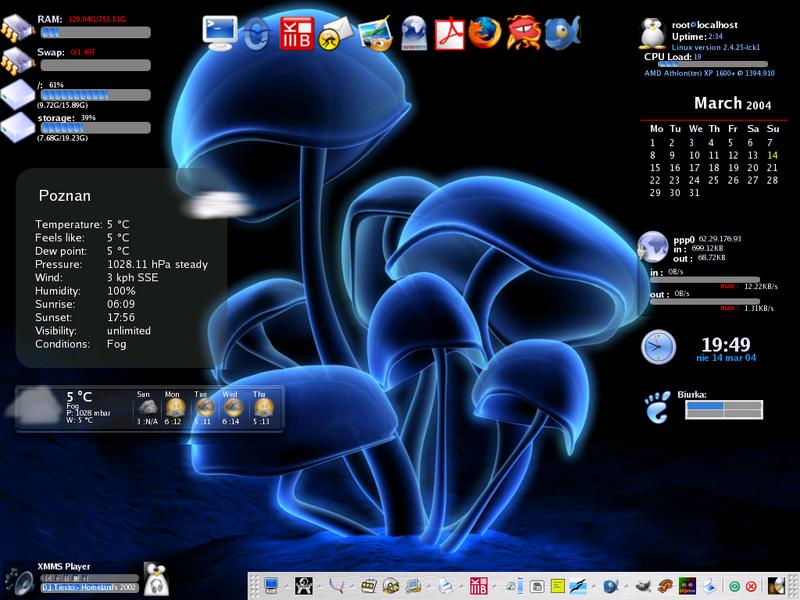
\includegraphics[height=3.5cm]{img/C03_estructura/gui_xfce}}
	\subfigure[LXDE]{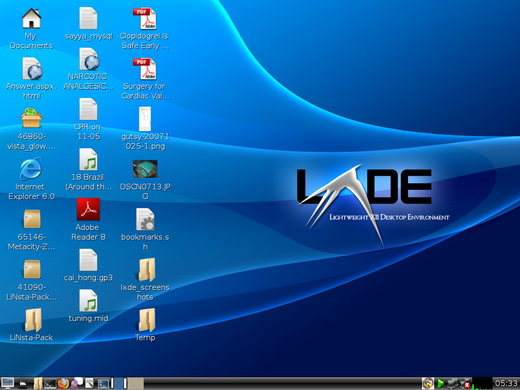
\includegraphics[height=3.5cm]{img/C03_estructura/gui_lxde}}
	\subfigure[Fluxbox]{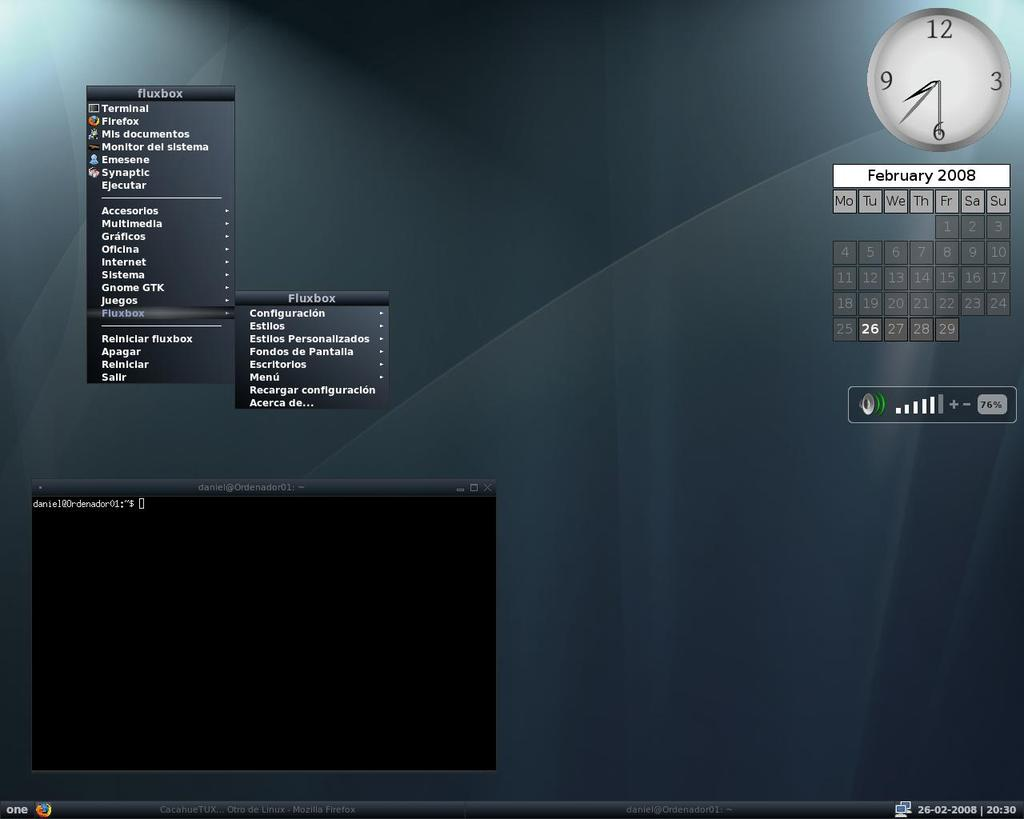
\includegraphics[height=3.5cm]{img/C03_estructura/gui_fluxbox}}
\end{center}
\caption{Diversos entornos gráficos}
\label{gui}
\end{figure}

\section{API y llamadas al sistema}
Las \textbf{llamadas al sistema} corresponden a una interfaz para utilizar los
servicios del sistema operativo, algunos ejemplos de estos son:

\begin{itemize}

	\item Errores de procesos (hardware o software).

	\item Lectura, creación o borrado de archivos.

	\item Imprimir texto por pantalla.

	\item Acceso a dispositivos de E/S.

\end{itemize}

Una \textbf{API} o \textit{Aplication Program Interface} corresponde al conjunto
de intrucciones y procedimientos que se ofrecen como biblioteca. En el caso del
sistema operativo, es la biblioteca que entrega las funciones que permiten hacer
uso de las llamadas al sistema.

La API es dependiente del sistema operativo, y algunos ejemplos de estas son la
API POSIX\footnote{Portable Operating System Interface, utilizada en sistemas
\textit{like Unix}}, la API Win32 y la API de Java.

La principal ventaja de utilizar una API para el desarrollo de aplicaciones
tienen que ver con la abstracción que el programador realiza del sistema, donde
no necesita conocer a fondo el mismo y puede generar una menor cantidad de
código e instrucciones más simples. Lo anterior implica una mayor facilidad al
momento de portar el código desde un sistema operativo (o máquina) a otro(a).

\subsection{Tipos de llamadas al sistema}
Las llamadas a sistemas se pueden dividir en cinco grupos principales, los
cuales corresponden a control de procesos, manipulación de archivos,
manipulación de dispositivos, mantenimiento de información y comunicaciones.
Estas serán discutidas a continuación.

\subsubsection{Control de procesos}
Estas llamadas a sistema se encargan de diferentes tareas que tienen relación
con los estados y vida de un proceso.

Por ejemplo se debe manejar el \textbf{término} donde en caso de errores se
podrá producir un volcado de memoria y el programador deberá proceder a depurar
el programa, por ejemplo utilizando una herramienta como gdb. En el caso de
término el sistema operativo deberá pasar a la siguiente tarea a realizar,
generalmente planificando un nuevo proceso. En caso del retorno de salida,
existen distintos niveles de error, donde el estándar es que 0 corresponde a un
retorno normal y cualquier valor positivo a un error, donde entre más alto el
número más grave debiese ser el error.

También se deben manejar temas relacionados con la \textbf{carga y ejecución}
del proceso, donde puede ser necesario cargar y/o ejecutar otro programa, por
ejemplo cuando un proceso $A$ llama a un proceso $B$. Una vez termina la
ejecución del proceso $B$ el control debería volver al proceso $A$. Esto último
se observa claramente al ejecutar un comando en un intérprete, ya que al
ejecutar, por ejemplo, el comando $ls$ cuando este termine el control volverá al
intérprete.

Otra llamada al sistema tiene relación con los \textbf{atributos de procesos},
donde el sistema operativo deberá obtener y fijar los mismos, como prioridad o
tiempo máximo de ejecución del proceso. \textbf{Tiempos de espera} los cuales
son determinados por un tiempo $X$ de espera o bien por la espera de algún
suceso que se requiera. O llamadas al sistema para la asignación de
\textbf{memoria principal}.

La llamada al sistema \textbf{\textit{kill}} permite enviar señales a los
procesos. Estas señales envían una instrucción al proceso con diferentes
objetivos, por ejemplo para matar el proceso (KILL), terminar el proceso (TERM),
suspender el proceso (STOP) o ejecutar una alarma (ALRM). Para enviar una señal
en sistemas \textit{like Unix} se utiliza el comando \textit{kill}.

Algunos ejemplos de llamadas al sistema relacionadas son \texttt{fork} (crea un
proceso hijo), \texttt{exec} (carga programa en memoria y ejecuta),
\texttt{wait} (espera hasta la finalización del proceso hijo) y \texttt{exit}
(termina la ejecución del proceso).

\subsubsection{Manipulación de archivos}
Las llamadas a sistema relacionadas con la manipulación de archivos tienen
principalmente las funciones de realizar \textbf{operaciones básicas sobre
archivos} y \textbf{determinar atributos o cambiarlos}, como el nombre el tipo
del archivo, los permisos que tiene un usuario, etc.

Algunos ejemplos de llamadas al sistema relacionadas son \texttt{create},
\texttt{delete}, \texttt{open}, \texttt{read}, \texttt{write},
\texttt{reposition} y \texttt{close}.

\subsubsection{Manipulación de dispositivos}
Permiten controlar el acceso a los dispositivos, el cual debe ser controlado, si
un proceso requiere un recurso y este está ocupado el proceso deberá esperar por
el recurso.

Los dispositivos que se deberán manipular pueden ser tanto físicos, como el
disco duro, y virtuales, como archivos. En sistemas \textbf{like Unix} los
dispositivos pueden ser encontrados en el directorio \texttt{/dev}.

Algunos ejemplos de llamadas al sistema relacionadas son \texttt{request},
\texttt{release}, \texttt{open}, \texttt{close}, \texttt{read}, \texttt{write} y
\texttt{reposition}.

\subsubsection{Mantenimiento de información}
El propósito de estas llamadas al sistema es transferir datos entre el programa
de usuario y el sistema operativo. Ejemplos de estos tipos de datos son tiempo,
usuarios, versión S.O., memoria libre (o disco duro), etc. Información general
del funcionamiento del sistema operativo puede ser encontrada, en sistemas
\textit{like Unix}, en el directorio \texttt{/proc}.

Algunos ejemplos de llamadas al sistema relacionadas son \texttt{time},
\texttt{date} y \texttt{sysinfo} (usada por comando \texttt{uname}).

\subsubsection{Comunicaciones}
En este tipo de llamadas al sistema se incluyen aquellas que permiten realizar
la comunicación entre procesos, por ejemplo mediante el \textbf{modelo por paso
de mensajes}, usando sockets o el \textbf{modelo de memoria compartida}, donde
se debe eliminar la restricción del sistema operativo que protege datos en
memoria en el caso de proceso pesados.

Algunos ejemplos de llamadas al sistema relacionadas son \texttt{get\_hostid},
\texttt{get\_processid}, \texttt{open}, \texttt{close},
\texttt{accept\_connection}, \texttt{wait\_for\_connection},
\texttt{read\_message}, \texttt{write\_message}, \texttt{shared\_memory\_create}
y \texttt{shared\_memory\_attach}.

\section{Diseño}
Durante el diseño del sistema operativo se deberá considerar que los
dispositivos sean mapeados en la memoria del computador como si fuesen
posiciones en ella, si se lee en dicha dirección de memoria, en el fondo, se
accede al dispositivo en si, análogamente si se escribe en esa dirección de
memoria se hará escritura en el disco. Esto es básicamente los que sucede con
los ficheros que se encuentran en \texttt{/dev} que representan dispositivos
físicos de la máquina.

% ejemplo disco duro e interrupciones
Sigamos con el ejemplo del disco, una vez terminada la ejecución de la rutina
llamada para realizar la lectura no significa que se haya realmente terminado de
leer desde el disco. En realidad la rutina que se ejecuta es el comando que se
introduce para que se inicie la verdadera lectura y el disco tiene su propio
microcontrolador que se encarga de realizar la operación. La CPU consultará
entonces reiteradamente para verificar si se completo o no la lectura en un
ciclo conocido como \textit{busy-waiting}, esto es lo que sucedía originalmente
en los primeros sistemas operativos como ya fue discutido anteriormente en el
capítulo \ref{historia}. El problema de este enfoque es que se pierde tiempo
mientras se realiza la operación de lectura, alrededor de 10 [ms], donde no se
hace otro trabajo útil.

Mucho mejor podría ser ejecutar otros procesos, mientras se espera que se lea el
disco, y se obtengan los datos que requiere el proceso para continuar. En este
caso el proceso quedará bloqueado y deberá esperar a que el sistema operativo le
notifique que los datos solicitados ya se encuentran listos para su uso.

El uso de interrupciones permite al disco avisar a la CPU que la operación en
disco terminó, se suspende al proceso que está actualmente en la CPU y se
ejecuta una rutina para atender la interrupción. Esta rutina de atención informa
al proceso que lo solicitado del disco ya está disponible y se pasa el proceso a
un estado listo para esperar a ser planificado nuevamente.

Existe dentro del núcleo del sistema operativo un vector de interrupciones con
todas las posibles fuentes de las mismas, como de disco o las del
\textbf{cronómetro regresivo}.

Un proceso que se esta ejecutando podría acaparar la CPU, entonces el sistema
operativo utiliza la interrupción del cronómetro regresivo para interrumpir al
proceso que se está ejecutando, por ejemplo después de 10 o 100 [ms], y asignar
la CPU a otro proceso, con este mecanismo se implementan las \textbf{tajadas de
tiempo}. Si estas son suficientemente pequeñas el usuario tendrá la sensación
que todo avanza al mismo tiempo, o sea, ``ejecución en paralelo''.

Otros ejemplos de interrupciones son aquellas que ocurren al hacer divisiones
por 0 o la ejecución de instrucciones ilegales (código de operación indefinida,
operación que no existe en el procesador o operación privilegiada).

No confundir interrupciones con señales, estas son ``interrupciones virtuales''
y su ámbito es en los procesos. Cada proceso maneja su propio cronómetro
regresivo virtual. El núcleo tiene una agenda con todas las señales que debe
generar y revisa cual es la próxima que debe ocurrir y entonces el cronómetro
regresivo coloca la alarma a dicha señal que se requiere para dicho proceso.
Mandar una señal a un proceso implica activar el proceso para que este pueda
atender la señal.
% fin ejemplo interrupciones

Otro aspecto a considerar en el diseño del sistema operativo son los canales que
se utilizan para acelerar la entrada y salida de datos, que pueden ayudar a
transferir muy rápido los datos. Lo anterior se logra utilizando un mecanismo
del mismo hardware que permite hacer una transferencia directa entre
dispositivos y memoria. Una vez terminada la transferencia se genera una
interrupción que indica que los datos ya están en la memoria. Con lo anterior el
núcleo evita tener que mover los datos desde el dispositivo a la memoria, esta
tarea la realiza el canal. Estos canales son conocidos como DMA o \textit{Direct
Memory Access}, donde el dispositivo, a través de este mecanismo, accede
directamente a la memoria.

\subsection{Objetivos}
Se deben definir objetivos y especificaciones, por ejemplo el hardware que se
requerirá y el tipo de sistema operativo que se desea implementar. Estos se
dividirán en objetivos del usuario y objetivos del sistema.

El \textbf{usuario} esta preocupado por que el sistema operativo sea cómodo de
utilizar, fácil de aprender y usar, fiable, seguro y rápido.

El \textbf{sistema} esta preocupado por que el sistema operativo sea flexible,
fiable, libre de errores, eficiente, fácil de diseñar, implementar y mantener.

Los objetivos tanto de usuario como de sistema a veces pueden no ser
compatibles, por ejemplo, para ser muy eficiente, quizás se deba sacrificar
usabilidad. Por lo anterior es que se deberá encontrar un equilibrio entre los
objetivos de ambos lados.

\subsection{Políticas y mecanismos}
Se deben definir \textbf{políticas} que indicarán \textbf{¿qué hacer?} y
\textbf{mecanismos} que indicarán \textbf{¿cómo hacerlo?}. Es recomendable que
políticas y mecanismos se encuentren separados, esto permitirá tener una mayor
flexibilidad ya que si se desea modificar una se puede minimizar el impacto en
la otra.

Las políticas determinarán todas las decisiones que el sistema operativo debe
tomar. Por ejemplo si se debe o no asignar un recurso, deberá existir una
política que indique cuando se aceptará la asignación y cuando se rechazará.
Asociado a esta política debe ir un mecanismo que indique como hacer la
asignación o como indicar el rechazo.

\subsection{Requerimientos para protección de procesos}
La \textbf{protección de procesos} significa que un proceso no debería
interferir con otros procesos, un proceso que esta corriendo no debería poder
acceder a los datos que otro esta manipulando. Ejemplos de estos sistemas
operativos son Unix y Windows NT, y los derivados de ambos.

\subsubsection{Modo dual}
En esta forma de operación se deben implementar dos modos básicos en que el
sistema operativo debe funcionar. El primero corresponde al \textbf{\textit{user
mode}}, o modo usuario o no privilegiado, en donde se ejecutan todos los
procesos, incluyendo aquellos que son ejecutados por el usuario root. Este modo
tiene ciertas restriccioens que impiden que un usuario pueda ejecutar cualquier
instrucción o código en la máquina, por ejemplo la instrucción que permite
deshabilitar las interrupciones. Si este modo no existiese un proceso cualquiera
podría desactivar, por ejemplo, el cronómetro regresivo, y evitar que otros
ocupen la CPU. En este modo, dicha instrucción es privilegiada, por lo cual al
ejecutarse ocurriría una interrupción de software (interrupción de comando
ilegal).

Es importante notar que a pesar de estar en modo usuario uno si podría
desactivar las señales en procesos (no ignorar, desactivar), excepto la señal
KILL. Si el proceso recibe una señal, la interrupción asociada ocurrirá pero el
sistema operativo no la entregará al proceso hasta que estén habilitadas
nuevamente. Importante mencionar que solo se desactivan señales de ese proceso,
ya que al ser modo usuario un proceso no puede interferir con otro.

El otro modo corresponde al \textbf{\textit{kernel mode}}, modo sistema, modo
supervisor o modo privilegiado. En este modo todo es permitido, por ejemplo aquí
si se podrían desactivar las interrupciones. El núcleo es el único que corre
sobre modo sistema, incluyendo sus módulos. Importante mencionar que dentro del
núcleo no hay \textit{segmentation fault}, en caso de existir algún error podría
derivar en un \textit{kernel panic}, es por esta razón que solo el usuario root
puede cargar módulos al núcleo.

En la figura \ref{modo_dual} se ilustra cada una de las partes que están
involucradas en el modo usuario y el modo sistema en GNU/Linux. Las aplicaciones
de los usuarios y la API glibc corren sobre el modo usuario, mientras que las
llamadas a sistema, el núcleo y las instrucciones directas al hardware lo hacen
en modo sistema. Si un usuario requiere hacer uso de una llamada a sistema
deberá hacerlo a través de la API correspondiente, entonces el sistema operativo
concederá solo por la ejecución de esa parte del código acceso a modo sistema,
revocándoselo una vez la instrucción termine y siguiendo su ejecución en modo
usuario. Es importante destacar que un usuario normal no puede acceder
llamadas de sistema privilegiadas, se requiere ser usuario root para esto.

\begin{figure}[htbp]
\begin{center}
	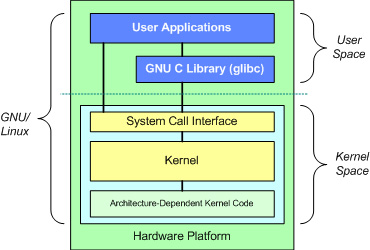
\includegraphics[scale=1.0]{img/C03_estructura/modo_dual}
	\caption{Componentes presentes en el modo usuario y el modo sistema}
	\label{modo_dual}
\end{center}
\end{figure}

\subsubsection{Unidad de gestión de memoria}

La \textbf{MMU} o \textit{Memory Management Unit} básicamente lo que hace es
traducir de direcciones virtuales a direcciones reales. Las direcciones
utilizadas por los procesos son virtuales, varios pueden usar la dirección 0x3A,
pero cuando se mapean a la memoria real se mapean a direcciones físicas
distintas, esto lo hace la MMU. Esto será cubierto en detalle en el capítulo
\ref{memoria_principal}.

Los primeros procesadores para computadores personales que aparecieron con MMU
fueron los x86, a mediados de los años 80s. Antes ya habían equipos con MMU,
pero eran los \textit{mainframes}\footnote{Computadoras grandes, potentes y
costosas utilizados en grandes instituciones}, ya que estos eran para
sistemas multiusuarios. Como ejemplo de sistemas operativos que la requieren
esta Unix que al ser multiusuario necesita MMU, Linux es derivado de Unix por lo
que también la requiere y Android al ser derivado de Linux igualmente la
necesita.

\section{Estructura del sistema operativo}
Se deberá elegir un método para estructurar las funcionalidades que se
proveerán. Actualmente los sistemas operativos se encuentran divididos por
jerarquías con funciones bien definidas. Se mencionarán algunas formas de
estructurar el sistema a continuación.

\subsection{Estructura simple}
La estructura simple esta orientada a sistemas operativos pequeños, simples y a
su vez limitados.

Por ejemplo, MS-DOS entregaba máximas funcionalidades en un tamaño reducido, no
poseía una división cuidadosa de sus módulos. Adicionalmente dicho sistema
operativo entregaba acceso directo a rutinas que podían utilizar el hardware,
por lo cual no se considera un sistema operativo con protección de sus procesos.

En el caso del Unix original, el kernel a través de las llamadas al sistema
provee las funcionalidades necesarias para acceder a los recursos.

\subsection{Estructura en niveles}
En este tipo de estructuras se utiliza un método de diseño arriba-abajo, el
sistema resultante corresponderá a un sistema por niveles donde la estructura
jerárquica se determinará de acuerdo a la complejidad de las funciones de cada
nivel.

Las ventajas de utilizar esta estructura radica en la independencia que se
conseguirá entre los niveles, ya que cada uno se encargará de una tarea
específica que le entregará servicios a otro nivel. Se debe preocupar mantener
las mismas funcionalidades que se entregan a otras capas, no importando como se
cambie esto internamente. Esto proporciona facilidad en la construcción,
mantención y depuración del sistema operativo.

Se debe tener especial cuidado en la definición apropiada de los diferentes
niveles, donde esto debe hacerse de forma correcta para lograr la independencia
anteriormente mencionada. Además se debe considerar que ciertas capas podrán
depender de otras para operar. Una desventaja es que al introducir niveles la
operación total podría resultar un poco más lenta, ya que se deben utilizar
interfaces entre las diferentes capas del sistema.

A continuación se muestra un ejemplo de los posibles niveles de jerarquía para
un sistema operativo. Notar los niveles del 1 al 4 no corresponden directamente
a funciones del sistema operativo, estas son realizadas por hardware. También
observar que las capas superiores requerirán servicios de capas inferiores como
es el caso del nivel de directorios que requiere servicios de la capa sistema de
archivos y esta a su vez de la capa de almacenamiento secundario.

\begin{enumerate}

	\item Circuitos electrónicos: registros, puertas, buses.

	\item Instrucciones: evaluación de la pila, microprogramas, vectores de
	datos.

	\item Procedimientos: pila de llamadas, visualización.

	\item Interrupciones: manejo de interrupciones del hardware.

	\item Procesos primitivos: semáforos, colas de procesos.

	\item Almacenamiento secundario: bloques de datos.

	\item Memoria virtual: paginación.

	\item Comunicaciones: tuberías.

	\item Sistema de archivos: almacenamiento en disco duro u otro medio.

	\item Dispositivos: impresoras, pantallas, teclados.

	\item Directorios: árbol de directorios.

	\item Procesos de usuario: programas en ejecución.

	\item Shell: intérprete de comandos.

\end{enumerate}

\subsection{\textit{Microkernels}}
Un sistema operativo que está organizado como micro núcleo entrega solo las
tareas básicas, como: planificación de procesos, gestor de memoria y
comunicaciones. Otras tareas son realizadas por programas del sistema operativo
y el núcleo es utilizado como un intermediario para la comunicación entre el
usuario y los programas del sistema operativo que ofrecen los servicios.

Los programas nuevos para el sistema operativo son añadidos al espacio del
usuario, se ejecutan en modo usuario y no como modo sistema. El núcleo entonces
se encarga de realizar las llamadas al sistema a través de mensajes hacia los
servicios correspondientes que entregan las funcionalidades solicitadas.

Su ventaja es que al incorporar las mínimas funcionalidades, son más estable.
Sin embargo la principal desventaja en este tipo de núcleos es que son
ineficientes al tener que realizar muchos cambios de contexto para ir a los
servicios prestados.

Minix es un ejemplo de este tipo de sistema operativo.

\subsection{Módulos}
En este caso el sistema operativo está compuesto por módulos, donde lo
fundamental se encuentra en el núcleo en si, pero otras funcionalidades son
entregadas como módulos del núcleo. Ambos, tanto el núcleo como los módulos
corren en modo sistema.

Esto permite que componentes sean cargados dinámicamente al núcleo, evitando
tener que disponer del soporte para todos los dispositivos o funcionalidades
permanentemente cargados en memoria principal. En Linux esto se puede realizar
mediante el uso de las instrucciones \texttt{lsmod}, \texttt{modprobe} y
\texttt{rmmod}.

Algunos ejemplos de módulos que pueden existir son controladores de disco,
controladores de tarjetas de red o el soporte para IPv6. Es importante mencionar
que el soporte necesario para que la máquina pueda ser arrancada, en estricto
rigor para que el disco duro que contiene el sistema raíz del sistema operativo
sea abierto, no puede ir como módulo del núcleo. Lo anterior ya que los módulos
se cargan cuando el sistema esta iniciando, una vez que ya se montó el sistema
de archivos.

Ejemplos de estos sistemas operativos son Unix modernos, Solaris, Linux y Mac
OSX.

Se hablará más adelante de módulos en Linux en el capítulo \ref{linux_modulos}.

\section{Implementación}
Una vez se decide la estructura del sistema operativo y están definidas las
políticas del mismo se debe realizar la implementación. Originalmente esto se
realizaba programando el hardware de la máquina, posteriormente se utilizaba un
lenguaje de bajo nivel o lenguaje de máquina (\textit{assembler}) y actualmente
se utilizan lenguajes de alto nivel (como C o C++).

La principal ventaja de utilizar lenguajes de alto nivel radica en que es fácil
de programar, el código que se escribe es compacto, fácil de entender y depurar.
Adicionalmente las mejoras introducidas en los compiladores significarán mejoras
en el código generado, por lo tanto mejoras en el sistema operativo que se está
compilando. Finalmente colabora con la portabilidad de un sistema operativo de
un hardware a otro, recordar que será la API de cada lenguaje la que se
encargará de traducir las instrucciones a la arquitectura seleccionada.

Desde el punto de vista de la optimización del sistema operativo es recomendable
atacar a las estructuras de datos y algoritmos utilizados en tareas críticas,
tales como el planificador de la CPU y el gestor de memoria. Una vez
identificados los problemas se deben optimizar, por ejemplo reemplazando el
código de alto nivel por código de máquina.

\section{Ejercicios y preguntas}
\begin{enumerate}

	\item Mencione y explique 5 servicios que se deben considerar al momento
	de diseñar el sistema operativo.

	\item ¿Cuál es la diferencia entre CLI y GUI?.

	\item Mencione tres ventajas de utilizar una API.

	\item ¿Qué es una llamada al sistema?, de dos ejemplos (que no sea
	kill).

	\item La llamada sistema kill permite enviar señales a procesos, indique
	la diferencia entre la señal KILL y TERM.

	\item ¿Por qué \textit{busy-waiting} es ineficiente?.

	\item ¿Quién atiende las interrupciones?.

	\item ¿Para que es utilizado el cronómetro regresivo?.

	\item Explique la diferencia entre interrupciones y señales.

	\item Explique el concepto de modo dual, o sea, explique los modos
	usuario y sistema. Adicionalmente de ejemplos de cuando se utiliza cada
	uno de ellos.

	\item ¿Cuándo ocurre un cambio de modo usuario a modo sistema?.

	\item ¿Una aplicación puede ejecutar directamente una llamada al sistema
	sin utilizar una API?

	\item Explique la estructura de núcleo monolítico.

	\item Explique la estructura de \textit{microkernels}.

	\item Linux ¿a que tipo de estructura de sistema operativo corresponde?.

	\item ¿Cuál es la ventaja de utilizar un sistema con estructura
	modular?.

\end{enumerate}

\section{Referencias}
\begin{itemize}

	\item Sistemas Operativos, Segunda Edición, Andrew Tanenbaum, Capítulo
	1.3, 1.4 y 1.5.

	\item Sistemas Operativos, Quinta Edición, Abraham Silberschatz y Peter
	Baer Galvin, Capítulo 3.

\end{itemize}


% CAPÍTULO 4: PROCESOS
%
% Apunte de Sistemas Operativos
% Copyright (C) 2014 Esteban De La Fuente Rubio (esteban[at]delaf.cl)
%
% Permission is granted to copy, distribute and/or modify this document
% under the terms of the GNU Free Documentation License, Version 1.3
% or any later version published by the Free Software Foundation;
% with no Invariant Sections, no Front-Cover Texts, and no Back-Cover Texts.
% A copy of the license is included in the section entitled "GNU
% Free Documentation License".
%
% Link: http://www.gnu.org/copyleft/fdl.html
%

% CAPÍTULO PROCESOS
\chapter{Procesos}
\label{procesos}
La definición más simple para describir un proceso corresponde a un
\textbf{programa en ejecución}. Es importante notar que el proceso no es solo el
código, sino que es el código más los datos que conforman al proceso, su pila,
registros del procesador, descriptores de E/S, etc, en general cualquier dato
que permita administrar el proceso. Veremos que esto último es conocido como
contexto del proceso.

Adicionalmente se debe considerar que un proceso para ser ejecutado, deberá ser
planificado por el sistema operativo, de esta forma podrá hacer uso de la CPU
por un período determinado de tiempo. Lo anterior ocurre ya que el proceso
está siendo ejecutado con otros procesos y debe compartir los recursos,
incluyendo la CPU.

\section{Distribución de la memoria}
Todo proceso que se ejecuta dentro del sistema operativo, utilizando una MMU,
verá direcciones virtuales. En estas direcciones virtuales se ordena la memoria
del proceso a partir de las direcciones más bajas como se muestra en la figura
\ref{fig:memoria_proceso}.

\begin{itemize}

	\item \textbf{Código del programa}: instrucciones en código de máquina a
	ejecutar por el proceso.

	\item \textbf{Datos}: área para variables globales, inicializadas o no
	inicializadas.

	\item \textbf{\textit{Stack}}: área para datos de funciones.

	\item \textbf{\textit{Heap}}: espacio utilizado para la asignación
	dinámica de memoria, por ejemplo mediante \texttt{malloc}.

\end{itemize}

Existen implementaciones donde el \textit{stack} y el \textit{heap} están
invertidos y el \textit{stack} crece hacia las direcciones  bajas de la memoria
virtual.

\begin{figure}[htbp]
\centering
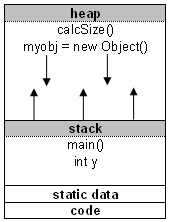
\includegraphics[scale=1.00]{img/C04_procesos/HeapAndStack}
\caption{Distribución de la memoria}
\label{fig:memoria_proceso}
\end{figure}

Las direcciones virtuales que no se encuentran asignadas al proceso, o sea
donde no hay un mapeo de dichas direcciones virtuales a direcciones físicas no
se pueden utilizar. Por lo cual si un proceso trata de acceder arbitrariamente
a una zona ilegal de memoria, donde no hay asignación o en algunos sistemas al
área del código se producirá una \textbf{\textit{segmentation fault}}. A
continuación se muestra un ejemplo de código que podría generar este error:

\lstinputlisting{codigo/C04_procesos/segmentation_fault.c}

En caso de un \textit{segmentation fault} el sistema generará una interrupción
llamada dirección ilegal, el sistema operativo determina la causa y envía una
señal al proceso indicando el error ocurrido. Si esta señal no es capturada por
el proceso hijo, entonces el proceso padre, muchas veces la \textit{shell},
recibirá la señal y mostrará el mensaje ``Segmentation fault'', el proceso hijo
terminará y el padre (\textit{shel}) continuará su ejecución.

En direcciones virtuales superiores, se encuentra la memoria del sistema, la
cual es solo accesible en modo sistema. Cuando ocurre una interrupción, el
núcleo atrapará la interrupción y el sistema operativo ejecutará, según el
vector de interrupciones, las instrucciones que atienden dicha interrupción.
Esta parte de la memoria, corresponde al núcleo del sistema operativo la cual
esta siempre residente en memoria y es ``compartida'' entre los procesos. Un
proceso normal no puede ver el área de código del sistema operativo, solo se
accede cuando hay un cambio a modo sistema. Ningún código que no pertenezca al
sistema deberá ejecutarse en dicha área de memoria, ya que de hacerlo implicaría
ejecución en modo sistema.

\section{Contexto}
El sistema operativo para gestionar el sistema requiere de diferentes datos, los
cuales se organizan en \textit{tablas}, ejemplo de estas tablas son:

\begin{enumerate}[i.]

	\item \textbf{Tabla de memoria}: asignación de memoria principal (RAM),
	asignación de memoria secundaria (almacenamiento), atributos de
	protección o de compartición y datos para la gestión de memoria virtual.

	\item \textbf{Tabla de E/S}: disponibilidad de recursos, estado de las
	operaciones de E/S y porción de memoria principal usada como
	origen/destino (\textit{buffers de E/S}).

	\item \textbf{Tabla de archivos}: existencia de archivos, posición en
	memoria secundaria, estado actual y otros atributos.

	\item \textbf{Tabla de procesos}: contexto del proceso.

\end{enumerate}

De esta última tabla, la de procesos, nos preocuparemos a continuación.

El \textbf{contexto}, imagen o descriptor del proceso corresponde a todos los
datos que el sistema operativo requiere para realizar la administración del
proceso. Este contendrá diversos datos referentes al estado de ejecución
del proceso.

El contexto será una estructura de datos que representará al proceso,
conteniendo datos del mismo, como por ejemplo cuantos milisegundos de CPU ha
usado el proceso en modo sistema o en modo usuario. El comando \texttt{time}
entrega el tiempo en modo usuario (\textit{user}) y modo sistema (\textit{sys}).
Las interrupciones que ocurren son contabilizadas en el tiempo del proceso que
ocurren, las cuales no necesariamente son del proceso que se esta ejecutando.
Un ejemplo de ejecución del comando time para un proceso de compilación es el
siguiente:

\begin{verbatim}
$ time gcc -Wall codigo.c -o programa
real    0m0.082s
user    0m0.052s
sys     0m0.020s
\end{verbatim}

\subsection{Atributos del proceso}
A continuación se listan algunos de los elementos que pueden ser encontrados
dentro del contexto de un proceso.

\subsubsection{Identificación del proceso}
\begin{itemize}

	\item Identificador del proceso.

	\item Identificador del proceso padre.

	\item Identificador del usuario.

\end{itemize}

El identificador del proceso o \textbf{PID} corresponde a la identificación
pública de un proceso. El Sistema operativo administra una tabla que permite
asociar el PID hacia la dirección donde se encuentra el contexto del proceso.
Los procesos entre sí se conocen únicamente por su PID.

\subsubsection{Información del estado del procesador}
\begin{itemize}

	\item Registros visibles para el usuario: aquellos que se pueden
	referenciar mediante el lenguaje de máquina.

	\item Registros de control y estado: aquellos utilizados por el
	procesador para ejecutar el código, ej: \textit{program counter}.

	\item Punteros de pila: apunta a la cima de la pila.

\end{itemize}

\subsubsection{Información de control del proceso}
\begin{itemize}

	\item Información de planificación y estado: estado, prioridad, sucesos
	u otros.

	\item Estructuración de datos: enlaces entre procesos, ejemplo:
	colas por estar bloqueados.

	\item Comunicación entre procesos: señales, mensajes, tuberías.

	\item Privilegios: memoria, tipo de instrucciones, servicios o
	utilidades del sistema.

	\item Gestión de memoria: punteros hacia las direcciones de memoria
	asignadas.

	\item Propiedad sobre recursos: recursos controlados por el proceso,
	ejemplo: archivos abiertos.

\end{itemize}

\subsection{Cambios de contexto}
El \textbf{cambio de contexto} de un proceso ocurre cuando el proceso que se
está ejecutando sale de la CPU y entra uno nuevo. Lo anterior ya que cada
proceso necesita su propio contexto para la ejecución del mismo, por lo cual el
que está almacenado debe ser limpiado y cargado el nuevo.

Si un proceso está ejecutando operaciones de entrada y salida, y los datos
asociados a estas operaciones no están en \textit{buffers} el proceso no
puede continuar, por lo cual debe bloquearse, entregar el control al sistema
operativo y el \textit{scheduler} tomará el control escogiendo otro proceso que
si pueda continuar, en ese momento ocurre un cambio de contexto entre los
procesos (el que sale por estar bloqueado y el que entra por estar listo). Lo
mismo ocurre cuando se acaba el tiempo mediante la interrupción del cronómetro
regresivo, ya que al no poder seguir usando la CPU el proceso debe salir y
entrar uno diferente (asumiendo que hay más procesos listos).

Suponga el siguiente escenario: tiene un proceso en ejecución en la CPU al cual
todavía le queda tiempo del asignado, sin embargo el sistema operativo debe
atender una interrupción que llegó por alguna razón. Al ser una interrupción el
proceso en ejecución será interrumpido y se pasará a ejecutar la parte de código
en el área de sistema, todo esto en el tiempo de ejecución del proceso que está
en la CPU. Luego de atender la interrupción se continuará con el proceso por el
tiempo que le queda disponible.

Es importante mencionar que una interrupción podría originar un cambio de
contexto, pero no necesariamente. Por ejemplo en el caso del cronómetro
regresivo se generará una interrupción que implicará cambio de contexto, pero
un aviso del disco duro enviando una interrupción informando que los datos
están ubicados en el \textit{buffer} no generará cambio de contexto. De todas
formas siempre esto tiene que ver con las políticas y mecanismos ya que un
sistema operativo podría generar un cambio de contexto ante una interrupción que
otro no lo genera.

Los cambios de contexto son caros ya que se debe limpiar la memoria donde
se almacena el mismo, y esto al acceder al hardware, es lento. Luego de limpiar
se debe restaurar el contexto de interés (escribiendo en la memoria).

Al realizar un cambio de contexto se debe:
\begin{itemize}

	\item Resguardar los registros del proceso que sale.

	\item Contabilizar el uso de CPU.

	\item Cambiar de espacio de direcciones virtuales. Usualmente implica
	invalidar caché de nivel 1, lo cual es lo más costoso, esto es así en
	los procesos pesados y deben su nombre justamente a esto.

	\item Resguardar los registros del proceso que entra.

\end{itemize}

\section{Estados}
Durante la ejecución de un proceso este puede encontrarse en diferentes estados,
se debe comprender que el proceso al iniciar su ejecución no siempre se estará
\textit{ejecutando}, ya que deberá compartir el tiempo de CPU con otros procesos
en el sistema, e inclusive con el mismo sistema operativo, el cual también es un
proceso en ejecución. Adicionalmente pueden ocurrir otras situaciones que lleven
al proceso de un estado a otro.

Los diferentes estados pueden ser vistos en la figura
\ref{fig:procesos_estados}. A continuación se describirán estos y los motivos
que pueden llevar a pasar de uno a otro durante la ejecución del proceso.

\begin{figure}[htbp]
	\centering
	\selectlanguage{english}
	\begin{tikzpicture}
		% formatos
		\tikzstyle{every node} = [auto, node distance=4cm, semithick]
		\tikzstyle{node} = [draw, circle, minimum size=3cm, very thick]
		\tikzstyle{arrow} = [->, very thick]
		% nodos
		\node [node] (inicio) {Inicio};
		\node [node] (listo) [below right of =inicio] {Listo};
		\node [node] (ejecucion) [right of =listo] {Ejecución};
		\node [node] (termino) [right of =ejecucion] {Término};
		\node [node] (bloqueado) [below of =listo] {Bloqueado};
		\node [node] (s_listo) [below left of =inicio] {Suspendido L.};
		\node [node] (s_bloqueado)[below of =s_listo] {Suspendido B.};
		% relaciones
		\draw [arrow] (inicio) to [bend left] node {} (listo);
		\draw [arrow] (inicio) to [bend right] node {} (s_listo);
		\draw [arrow] (s_listo) to [bend left] node {} (listo);
		\draw [arrow] (listo) to [bend left] node {} (s_listo);
		\draw [arrow] (listo) to [bend left] node {} (ejecucion);
		\draw [arrow] (ejecucion) to [bend left] node {} (listo);
		\draw [arrow] (ejecucion) to [bend left] node {} (termino);
		\draw [arrow] (ejecucion) to [bend left] node {} (bloqueado);
		\draw [arrow] (bloqueado) to [bend left] node {} (listo);
		\draw [arrow] (bloqueado) to [bend left] node {} (s_bloqueado);
		\draw [arrow] (s_bloqueado) to [bend left] node {} (bloqueado);
		\draw [arrow] (s_bloqueado) to [bend left] node {} (s_listo);
	\end{tikzpicture}
	\selectlanguage{spanish}
	\caption{Estados de un proceso}
	\label{fig:procesos_estados}
\end{figure}

Cuando se lanza un programa a ejecución, el proceso no necesariamente comienza a
ejecutarse inmediatamente, sino que pasará por un estado de \textbf{inicio},
donde se deberán realizar distintas operaciones que tienen que ver con la
preparación del entorno para la ejecución del proceso.

Una vez que se ha creado el entorno del proceso, y existe memoria para que este
pueda comenzar, pasa a estado \textbf{listo} donde espera a ser planificado para
entrar a la CPU y ejecutar su código.

Al momento de ser elegido el proceso para su ingreso a la CPU pasa a estado de
\textbf{ejecución}. Donde se encontrará, en una primera instancia, hasta que el
tiempo asignado por el sistema operativo expire. Una vez el tiempo expire el
proceso volverá a estado listo, donde volverá a esperar para ser planificado.

Si durante la ejecución del proceso este requiere algún recurso que no está
disponible, el proceso pasará a estado \textbf{bloqueado} hasta que el sistema
operativo le indique que el recurso que está solicitando le fue asignado. Como
se vió anteriormente, esto podría ser por ejemplo una lectura de datos desde el
disco. Una vez se asigna el recurso el proceso pasará a estado listo nuevamente
con el recurso ya disponible para ser utilizado la próxima vez que entre a la
CPU.

Una vez el proceso haya cumplido con la ejecución de su programa, o haya
ocurrido algún evento que lleve al proceso a su estado final, se encontrará en
estado de \textbf{término} o estado \textit{zombie}, donde el proceso ya terminó
su ejecución pero aun no se han liberado sus recursos. Esto es utilizado, por
ejemplo, por un proceso padre que requiere datos una vez el proceso haya
terminado, por lo cual será la llamada a \texttt{wait} del proceso padre la que
liberará finalmente los recursos del proceso \textit{zombie}.

Las razones de término de un proceso no solo se deben porque terminó con la
ejecución de su código, a continuación se mencionan otras causas:
\begin{itemize}
	\item Límite de ejecución excedido.
	\item Límite de espera excedido.
	\item No hay memoria disponible.
	\item Violación de segmento (o límites).
	\item Error de protección.
	\item Error aritmético.
	\item Error E/S.
	\item Instrucción inválida.
	\item Instrucción privilegiada.
	\item Mal uso de datos.
	\item Intervención del SO.
	\item Terminación del padre.
	\item Solicitud del padre.
\end{itemize}

Con los estados descritos hasta ahora un sistema podría funcionar, sin embargo
¿qué sucedería si en un determinado momento el sistema tiene muchos procesos
bloqueados y otros nuevos esperando entrar a estado listo? Con el esquema
descrito hasta ahora, si la RAM estuviese completamente ocupada nuevos procesos
no podrían ser recibidos. Considerando esto es que aparecen dos estados
adicionales, \textbf{suspendido listo} y \textbf{suspendido bloqueado}, los
cuales se encargarán de mover a un almacenamiento secundario los procesos que
por alguna razón no puedan ser llevados a estado listo. Si un proceso se
encuentra bloqueado será llevado a bloqueado suspendido para que espere sin
consumir RAM por el recurso que está solicitando, en cambio si un proceso es
nuevo y no hay memoria RAM podrá ser iniciado en un estado suspendido listo,
donde ya tendrá su contexto y solo faltará memoria principal para poder ser
candidato a planificación.

El sacar un proceso de la CPU y colocar otro en esta implicará diversos pasos,
los cuales se mencionan a continuación:
\begin{enumerate}

	\item Guardar el contexto del proceso que sale.

	\item Actualizar el bloque de control del proceso que sale.

	\item Mover el bloque de control a la cola adecuada (según estado en que
	quedó el proceso que sale).

	\item Seleccionar otro proceso para ejecución (planificación).

	\item Actualizar el bloque de control del proceso seleccionado (cambiar
	a ejecución).

	\item Actualizar las estructuras de datos de gestión de memoria.

	\item Restaurar el contexto del proceso, incluyendo los
	registros del procesador a aquel estado que existía cuando el proceso
	seleccionado dejó el procesador la vez anterior.

\end{enumerate}

Nos preocuparemos especialmente de los algoritmos de planificación más adelante.

\section{Clasificación de procesos}
Los procesos pueden clasificarse en dos grupos básicos, como \textbf{procesos
pesados} y como \textbf{procesos livianos}. Cada uno tendrá sus características,
ventajas y desventajas. En el cuadro \ref{tab:procesos_clasificacion} se pueden
apreciar sus similitudes y diferencias.

\begin{table}[hbt]
	\centering
	\begin{tabular}{|c|c|c|}
		\hline
						& Pesado			& Liviano \\
		\hline
			Jerga			& procesos Unix			& threads \\
			Implementación		& fork				& hebras \\
			Espacio de direcciones	& propio  			& compartido \\
			Archivos		& compartido			& compartido \\
			Procesador		& propio (1)			& propio (varios) \\
			Requisitos de hardware	& MMU, interrupciones y timers	& interrupciones y timers \\
			Protección		& si				& no \\
			Comunicaciones		& mensajes, sockets, pipes	& memoria compartida (punteros) \\
			Costo cambio contexto	& alto				& bajo \\
			Ejeplos	de S.O.		& Unix e IBM VM370		& AmigaOS, MacOS y Win 3.11 \\
		\hline
	\end{tabular}
	\caption{Comparativa entre procesos pesados y livianos}
	\label{tab:procesos_clasificacion}
\end{table}

Notar que la comparación se hace pensando en la ejecución de varios procesos
pesados en paralelo en un sistema operativo, o bien la ejecución de un único
proceso liviano con muchas hebras ejecutándose de forma paralela.

En sistemas operativos \textit{like Unix} tradicionalmente se han utilizado
procesos pesados. Si bien POSIX entrega una implementación de hebras, esto es
más ``moderno'', en los tiempos iniciales solo habían procesos pesados.

Sistemas operativos \textit{de juguete} por lo general utilizan procesos
livianos, ya que el sistema operativo en sí corre sobre un proceso pesado de
Unix.

Sistemas operativos como Unix modernos, Linux o WIndows 2000 y NT hacia adelante
pueden proveer tanto procesos pesados como livianos.

\subsection{Procesos \textit{preemptive} y \textit{non-preemptive}}
Adicionalmente a la clasificación anterior el sistema operativo puede ofrecer,
una de estás opciones, procesos de tipo \textit{preemptive} y
\textit{non-preemptive}.

\subsubsection{Procesos \textit{preemptive}}
Los procesos \textbf{\textit{preemptive}} son aquellos donde el núcleo puede
quitar la CPU a un proceso en cualquier momento, esto mediante interrupciones.

Ejemplos de este tipo de sistema son sistemas \textit{like Unix} y Windows NT y
posteriores.

\subsubsection{Procesos \textit{non-preemptive}}
En los procesos \textbf{\textit{non-preemptive}} es el proceso quien decide
invocar al núcleo y devolver el control al sistema operativo. En estos casos
debe haber una cooperación entre las aplicaciones y el sistema operativo para
ofrecer paralelismo.

Ejemplo de este tipo de sistema son Windows 3.11 y MacOS antes de la versión
6.X. Los sistemas operativos mencionados no estaban diseñados para la ejecución
simultánea de varias aplicaciones, siendo las aplicaciones quienes debían
implementar mecanismos de sincronización.

La principal ventaja de esta forma de ejecución de procesos es que son fáciles
de programar. Como desventaja se tiene que sin un proceso se queda en un
\textit{loop} infinito la única solución es reiniciar la máquina.

\section{Paralelismo}
Un sistema con multiprocesador será capaz de ejecutar procesos en paralelo, en
este caso se están considerando varios \textit{chips}. Otra alternativa
corresponde a un sistema multinúcleo, donde existe un solo chip de procesador el
cual posee varias CPU (núcleos).

En general, lo que hará el sistema operativo será emular el multiprocesamiento,
ya que si bien se puede contar con un procesador con 2 o 4 núcleos, o más,
siempre se querrá tener más procesos en ejecución que la cantidad de núcleos que
la máquina pueda proveer. En estos sistemas se entregarán tajadas de tiempo,
donde cada proceso dispondrá de un tiempo finito y determinado para ejecutar su
código, de no alcanzar deberá intentarlo más tarde nuevamente.

Si bien este paralelismo solo se podría lograr al disponer de un sistema con
múltiples procesadores se debe recordar que los tiempos son tan pequeños que al
ejecutarse todos los procesos da la sensación que ocurren en paralelo.

El concepto de concurrencia está relacionado con la ejecución en
\textit{paralelo} de los procesos. La \textbf{concurrencia} aparecerá al
ejecutarse procesos en paralelo, donde dos o más procesos querrán acceder al
mismo tiempo a un determinado recurso. Originalmente la única programación con
múltiples procesos era la del sistema operativo, ya que los lenguajes no
entregaban soporte para concurrencia. Pero hoy en día, como los lenguajes si
ofrecen concurrencia como parte del lenguaje o biblioteca es importante conocer
lo que esta implica.

Independientemente de si estamos trabajando en un sistema multiprocesador,
multinúcleo o con emulación del paralelismo existirán problemas relacionados a
este \textit{paralelismo}. Los cuales tendrán directa relación con la forma en
que se ejecutan los procesos. Se discutirán a continuación los problemas que
pueden ocurrir en un ambiente con múltiples procesos en ejecución, los cuales
corresponden a \textit{data races}, \textit{deadlocks} y \textit{starvation}. En
el capítulo \ref{sincronizacion} se verán métodos de sincronización que
permitirán controlar estas situaciones.

\subsection{\textit{Data races}}
Los \textbf{\textit{data races}} o condición de carrera (\textit{race
condition}) ocurre en un proceso cuando se obtiene un estado inconsistente del
sistema, o bien cuando los datos que se obtienen se encuentran en un estado
inconsistente. La idea de carrera se puede considerar como dos o más procesos
que compiten para producir cierto estado final del sistema.

Considere el siguiente código:
\begin{lstlisting}
/* parte global (comun a todos los hilos) */
int contador = 0;
/* codigo principal de cada hilo en ejecucion */
void aumentar ()
{
  int aux = contador; /* instruccion 1 */
  contador = aux + 1; /* instruccion 2 */
}
\end{lstlisting}

Suponga que la función \texttt{aumentar()} se está ejecutando en forma
paralela en dos hilos (hebras o \textit{threads}), ¿qué problema se podría
presentar?. Se debe considerar que las operaciones de la función no son
atómicas, o sea pueden ser divididas, por lo tanto el sistema operativo puede
interrumpir al proceso y detener su ejecución en cualquier línea de ejecución
del código\footnote{Se ha forzado el código a tener 2 líneas, sin embargo debe
considerar que aunque fuese una línea la operación será dividida en varias
operaciones al ser pasada a código de más bajo nivel}. Al existir la posibilidad
que el sistema operativo interrumpa la ejecución del código en cualquier parte
del código puede ocurrir la siguiente situación:

\begin{enumerate}[i.]

	\item Hilo 1 ejecuta la función \texttt{aumentar()}, guarda el
	valor del contador y es interrumpido. Entonces aux = 0.

	\item Hilo 2 ejecuta la función \texttt{aumentar()}, guarda el
	valor del contador y es interrumpido. Entonces aux = 0.

	\item Hilo 1 hace la suma y guarda el valor. Entonces contador = 1.

	\item Hilo 2 hace la suma y guarda el valor. Entonces contador = 1.

\end{enumerate}

Al final de la operación la variable contador tendrá el valor 1, ¿era el valor
esperado? ¿qué valor debiera tener la variable contador?.

El resultado esperado será inconsistente ya que se esperaba que después de la
ejecución de los dos hilos el contador tuviese valor 2. Sin embargo a causa de
la ejecución en paralelo y la no existencia de sincronización el valor
resultante es incorrecto. Este problema también es conocido como el problema de
\textbf{exclusión mutua}, ya que lo lógico que se esperaría es que mientras un
proceso modifica una sección crítica los otros no puedan hacerlo.

Este es, de los problema de concurrencia que se verán, el peor de todos ya que
son \textbf{difíciles de detectar} y son \textbf{no determinísticos}.
Adicionalmente entregan un resultado al usuario, uno incorrecto, con lo cual él
podría no darse cuenta si dicho resultado es o no el esperado.

\subsubsection{Agregar elementos a una pila o \textit{stack}}
\begin{lstlisting}
Pila p;
int indice = 0;
void agregar(Pila p, Objeto o)
{
  put(p, o, indice++);
}
\end{lstlisting}

\subsubsection{Sentarme en una silla}
\begin{lstlisting}
int sillas[10]; /* arreglo inicializado en 0 */
void sentarme ()
{
  int i;
  for(i=0; i<10; ++i) {
    if(sillas[i]==0) {
      sillas[i] = 1;
      me_siento(i);
      break;
    }
  }
}
\end{lstlisting}

Se debe evitar pensar que el orden de las instrucciones puede ayudar con los
problemas de \textit{data races}, ya que el compilador puede reordenar el código
secuencial dejándolo de una forma no deseada. La solución correcta es el uso de
alguna herramienta de sincronización, como semáforos, para garantizar la
exclusión mutua.

\subsection{\textit{Deadlock}}
Un \textbf{\textit{deadlock}} o interbloqueo corresponde a una situación donde
un proceso requiere cierto recurso que algún otro tiene asignado, pero el otro
proceso para continuar, y eventualmente liberar el recurso, requiere el que
tengo yo asignado. Esto se puede observar en la figura \ref{fig:interbloqueo}.

\begin{figure}[htbp]
	\centering
	\selectlanguage{english}
	\begin{tikzpicture}
		% formatos
		\tikzstyle{every node}=[auto, node distance=4cm, semithick]
		\tikzstyle{arrow} = [->, very thick]
		% nodos
		\node [draw, circle] (R1) {Recurso 1};
		\node [draw] (PA) [below left of =R1] {Proceso A};
		\node [draw] (PB) [below right of =R1]	{Proceso B};
		\node [draw, circle] (R2) [below right of =PA] {Recurso 2};
		% relaciones
		\draw [arrow] (R1) to node {asignado} (PA);
		\draw [arrow] (PA) to node {pide} (R2);
		\draw [arrow] (R2) to node {asignado} (PB);
		\draw [arrow] (PB) to node {pide} (R1);
	\end{tikzpicture}
	\selectlanguage{spanish}
	\caption{Interbloqueo, espera circular entre proceso A y B}
	\label{fig:interbloqueo}
\end{figure}

Supongamos por un momento que tenemos una función que permite solicitar un
recurso y otra que permite liberar el recurso, más adelante veremos que esto es
posible hacerlo mediante herramientas como los semáforos. En este escenario se
propone la siguiente situación, donde Pa y Pb son dos procesos diferentes y que
se están ejecutando de forma paralela.

\begin{lstlisting}
Pa                       Pb
solicitar(S);            solicitar(Q);
solicitar(Q);            solicitar(S);
/* uso de Q y S en la seccion critica */
devolver(S);             devolver(Q);
devolver(Q);             devolver(S);
\end{lstlisting}

Si el proceso A se está ejecutando, solicita $S$, lo sacan de la CPU, entra el
proceso B y solicita $Q$. ¿Qué sucedera cuando entre nuevamente A y solicite
$Q$?. Ambos procesos estarán esperando que el otro libere el recurso que
necesitan.

Pensando en un ejemplo más concreto podría corresponder al problema:
\begin{lstlisting}
Servicio tenedor;
Servicio cuchillo;
function comer_asado()
{
  solicitar(tenedor);
  solicitar(cuchillo);
  comer();
  liberar(tenedor);
  liberar(cuchillo);
}
\end{lstlisting}

Para comer se requiere tanto el tenedor como el cuchillo y solo hay disponibles
uno de cada uno. ¿Qué podría ocurrir al haber dos personas tratando de comer?

Otro ejemplo puede ser el del puente colgante, donde:
\begin{itemize}

	\item Tráfico en una sola dirección.

	\item Cada sección del puente será un recurso.

	\item Si ocurre un \textit{deadlock}, uno de los usuarios deberá
	retroceder.

	\item Puede ser que varios usuarios deban retroceder.

	\item Puede haber inanición.

\end{itemize}

Para que ocurra interbloqueo se requieren las siguientes condiciones:
\begin{enumerate}

	\item Debe existir exclusión mutua.

	\item Los procesos deben mantener tomado el recurso y esperar por el
	siguiente.

	\item No debe existir apropiación por parte del sistema operativo
	(o sea que pueda quitarles el recurso).

	\item La espera debe ser circular.

\end{enumerate}

A continuación se mencionan posibles casos con los que el sistema operativo
podrá enfrentar un interbloqueo.

\subsubsection{Ignorar el problema}
\begin{itemize}

	\item Hacer como si el problema no existiera.

	\item Fundamento: bloqueos pueden ocurrir muy pocas veces, donde las
	políticas para solucionarlo pueden llevar a mecanismos complejos y que
	degraden el rendimiento del sistema.

	\item Unix utiliza este mecanismo.

\end{itemize}

\subsubsection{Detección y recuperación}
\begin{itemize}

	\item Permite que ocurran bloqueos.

	\item Cuando ocurren los detecta y lleva a cabo una acción para
	solucionarlo.

	\item Detección: ejecutar algoritmo cada X tiempo que verifique si
	existen interbloqueos.

	\item Recuperación:
	\begin{itemize}

		\item Apropiación: quitar el recurso y asignarlo al otro
		proceso.

		\item Rollback: volver el sistema hacia un punto donde no hay
		bloqueo.

		\item Eliminación del proceso: se eliminan procesos hasta romper
		el bloqueo.

	\end{itemize}

\end{itemize}

\subsubsection{Evitarlo dinámicamente}
\begin{itemize}

	\item Se hace una simulación de como quedaría el sistema si se asigna un
	recurso solicitado por un proceso.

	\item Se considera un estado seguro (todos satisfacen sus
	requerimientos) y uno inseguro (si uno o más procesos no podrán verse
	satisfechos).

	\item Si el estado en que queda la simulación es insegura, los recursos
	no serán asignados al proceso y deberá esperar.

	\item Algoritmo difícil de implementar, ya que procesos no conocen sus
	necesidades de recursos para un estado futuro.

\end{itemize}

\subsubsection{Evitar las cuatro condiciones}
Se busca que al menos una de las 4 condiciones necesarias para el bloqueo no se
cumpla.
\begin{itemize}

	\item Exclusión mutua: si los recursos no se asignaran de forma
	exclusiva a un proceso no habría problema de interbloqueos.

	\item Retención y espera: se debe evitar que procesos que ya tienen
	asignados recursos puedan solicitar nuevos sin liberar los que ya tienen
	(al menos temporalmente).

	\item No apropiación: quitar el recurso y asignarlo a otro (no siempre
	aplicable, ejemplo: impresora).

	\item Espera circular: los procesos deberán ordenarse para solicitar los
	recursos, no pudiendo hacerlo todos al mismo tiempo.

\end{itemize}

\subsection{\textit{Starvation}}
Una situación de \textbf{\textit{starvation}}, hambruna o inanición corresponde
a la situación donde por alguna razón un proceso no obtiene nunca el recurso
solicitado. Finalmente el proceso termina por tiempo de espera excedido, o sea,
muere de hambre. La existencia de hambruna permitirá tener un mayor
paralelismo.

Un ejemplo de esta situación:
\begin{itemize}
	\item Procesos A, B y C.
	\item Recurso R.
	\item Planificador asigna recurso R a A y B, pero nunca a C.
	\item C nunca adquiere el recurso para completar su objetivo y muere.
\end{itemize}

Para manejar el problema de inanición el sistema operativo puede asignar los
recursos mediante una cola FIFO o bien utilizar una prioridad para los procesos,
penalizando a quienes han adquirido el recurso y favoreciendo a quienes no. Esto
lo que busca es una asignación equitativa de los recursos, donde ninguno de los
procesos debe quedar sin ser atendido.

\section{Ejercicios y preguntas}
\begin{enumerate}

	\item ¿Qué compone a un proceso?.

	\item ¿Cuándo se ejecuta en CPU un proceso?.

	\item ¿Para qué se utiliza el espacio de memoria \textit{heap}?.

	\item ¿Para que se utiliza el espacio de memoria \textit{stack}?.

	\item ¿Qué es un \textit{segmentation fault}?.

	\item Describa a que corresponde el descriptor de un proceso.

	\item ¿Qué es el PID de un proceso?.

	\item ¿Qué información guarda el registro de CPU PC (\textit{program
	counter})?.

	\item Explique el proceso de cambio de contexto.

	\item ¿Cuáles son los estados de un proceso?, no es necesario que
	considere estados suspendidos.

	\item ¿Cuándo se pasa de estado listo a ejecución?.

	\item ¿Cuándo se pasa de estado ejecución a bloqueado?.

	\item ¿Cuándo se pasa de estado bloqueado a listo?.

	\item Indique 5 razones de término de un proceso.

	\item ¿Por qué es necesario el estado \textit{zombie} o terminado?.

	\item ¿Qué se debe restaurar cuando un proceso pasa de estado listo a
	ejecución?.

	\item Explique los proceso pesados y livianos, con sus ventajas y
	desventajas.

	\item Explique la diferencia entre procesos \textit{preemptive} y
	\textit{non-preemptive}.

	\item ¿Bajo que condición existe paralelismo en un sistema operativo?.

	\item Explique el problema de \textit{data races}.

	\item Explique el problema de \textit{deadlock}.

	\item Explique el problema de \textit{starvation}.

	\item Explique dos medidas que se puedan tomar frente a un interbloqueo.

	\item ¿Por qué el problema de \textit{data races} es considerado el mas
	complicado (malo) de los tres?.

\end{enumerate}

\section{Referencias}
\begin{itemize}

	\item Sistemas Operativos, Segunda Edición, Andrew Tanenbaum, Capítulo
	2.1.

	\item Sistemas Operativos, Quinta Edición, Abraham Silberschatz y Peter
	Baer Galvin, Capítulo 4.

	\item Sistemas Operativos, Segunda Edición, William Stallings, Capítulo
	3.

\end{itemize}


% ANEXOS
\renewcommand{\appendixname}{Anexo}
\appendix

% ANEXO A: MÁQUINAS VIRTUALES
%
% Apunte de Sistemas Operativos
% Copyright (C) 2014 Esteban De La Fuente Rubio (esteban[at]delaf.cl)
%
% Permission is granted to copy, distribute and/or modify this document
% under the terms of the GNU Free Documentation License, Version 1.3
% or any later version published by the Free Software Foundation;
% with no Invariant Sections, no Front-Cover Texts, and no Back-Cover Texts.
% A copy of the license is included in the section entitled "GNU
% Free Documentation License".
%
% Link: http://www.gnu.org/copyleft/fdl.html
%

% MÁQUINAS VIRTUALES
\chapter{Máquinas virtuales}
Una máquina virtual entrega una abstracción del hardware de la máquina hacia el
sistema operativo, proporcionando una interfaz de hardware virtual similar a la
de la máquina real. Los discos duros son emulados, por ejemplo, mediante
imágenes de discos. El sistema operativo que corre sobre la máquina virtual
desconoce tal condición, o sea, no sabe que funciona sobre una máquina virtual y
no una real. Este tipo de sistemas permite correr múltiples sistemas operativos
sobre una misma máquina. Ejemplos de sistemas de virtualización son KVM, XEN y
VirtualBox.

El sistema operativo que corre sobre la máquina virtual también posee un modo de
ejecución usuario y de sistema, sin embargo estos son modos virtuales que corren
sobre un modo usuario real. Esto significa que si en el sistema operativo
virtual hay una solicitud a una llamada del sistema a través de un programa que
corre en modo usuario virtual, esta será procesada por el sistema operativo en
modo sistema virtual y se entregará a la máquina virtual, la cual, en modo
usuario real, atenderá la interrupción mediante el hardware virtualizado y
entregará la respuesta al sistema operativo. En caso que se requiera acceso al
hardware real, la máquina virtual deberá hacer uso de la API del sistema
operativo real para acceder al recurso solicitado.

Es importante mencionar que los tiempos de respuesta en máquinas virtuales serán
más lentos que en máquinas reales. Lo anterior debido a la emulación que se debe
realizar del hardware y por la posibilidad de que existan múltiples máquinas
virtuales en ejecución en un mismo sistema real.

Las principales ventajas de esta solución es que permite realizar una protección
por aislamiento de los recursos del sistema, ya que el sistema virtualizado solo
verá dispositivos virtuales y en caso de cualquier problema solo podrá afectar a
la máquina virtual quedando la máquina real protegida. Adicionalmente son un
medio ideal para la realización de pruebas de sistemas operativos, como la
prueba de módulos en desarrollo o la prueba de servicios que se desean
implementar en una máquina real. También permiten aprovechar mejor el hardware
disponible, entregando servicio en un mismo equipo a diferentes sistemas
operativos que en conjunto comparten de forma eficiente el hardware disponible.


\end{document}
